\documentclass [MAS] {uclathes}

% \input {mymacros}                         % personal LaTeX macros

%%%%%%%%%%%%%%%%%%%%%%%%%%%%%%%%%%%%%%%%%%%%%%%%%%%%%%%%%%%%%%%%%%%%%%
%
% Usually things live in separate flies.
%
% \input {prelim}                           % preliminary page info

%%%%%%%%%%%%%%%%%%%%%%%%%%%%%%%%%%%%%%%%%%%%%%%%%%%%%%%%%%%%%%%%%%%%%%%%
%                                                                      %
%                          PRELIMINARY PAGES                           %
%                                                                      %
%%%%%%%%%%%%%%%%%%%%%%%%%%%%%%%%%%%%%%%%%%%%%%%%%%%%%%%%%%%%%%%%%%%%%%%%

\title          {An Application of Split-Attention Networks:\\
                Melanoma Detection}
\author         {Andrew Amir Ali Mashhadi}
\department     {Statistics}
\degreeyear     {2023}

%%%%%%%%%%%%%%%%%%%%%%%%%%%%%%%%%%%%%%%%%%%%%%%%%%%%%%%%%%%%%%%%%%%%%%%%

\chair          {Yingnian\ Wu}
\member         {Frederic Paik\ Schoenberg}
\member         {Michael Tsiang}

%%%%%%%%%%%%%%%%%%%%%%%%%%%%%%%%%%%%%%%%%%%%%%%%%%%%%%%%%%%%%%%%%%%%%%%%

\abstract       {

Melanoma is one of the most aggressive forms of skin cancer. In 2023 alone, the American Cancer Society estimates that about 7,990 Americans will die from new melanoma cases. Image analysis tools that automate the diagnosis of melanoma will improve dermatologists' diagnostic accuracy and should provide a significantly better detection of melanoma. 

In this paper, we present an application of modern deep learning architectures using the images of skin lesions in combination with patient-level contextual information to detect the presence of melanoma. More specifically, we used the latest variant of the residual network, the ResNeSt model, to leverage its deep architecture and channel-wise attention mechanisms for melanoma detection. In parallel, we used a multi-layer perceptron model to process patient-level data, and fused its output with the extracted features from the ResNeSt model. To compare and contrast performances, we trained a similar model using a smaller, more generic, convolutional neural network in addition to the larger ResNeSt network. After properly tuning all associated hyperparameters, our primary model obtained a balanced accuracy of 0.853 and a ROC-AUC score of 0.93. The split-attention network was shown to improve the total ROC-AUC by approximately 9\%, suggesting that our model was able to successfully leverage the ResNeSt design to extract the most important features and most relevant cross-feature interactions for the detection of melanoma.}

%%%%%%%%%%%%%%%%%%%%%%%%%%%%%%%%%%%%%%%%%%%%%%%%%%%%%%%%%%%%%%%%%%%%%%%%

\usepackage{subcaption} 
\usepackage{graphicx}
\usepackage{amsmath}
\usepackage{amsfonts}
\usepackage{array, makecell}
\usepackage{multirow}
\renewcommand\cellset{\renewcommand\arraystretch{0.8}%
\setlength\extrarowheight{0pt}}

%%%%%%%%%%%%%%%%%%%%%%%%%%%%%%%%%%%%%%%%%%%%%%%%%%%%%%%%%%%%%%%%%%%%%%%%

\begin {document}

\makeintropages

%%%%%%%%%%%%%%%%%%%%%%%%%%%%%%%%%%%%%%%%%%%%%%%%%%%%%%%%%%%%%%%%%%%%%%%%

\chapter{Introduction}

\section{Background}

In the past decade, machine learning has exploded in popularity. Machine learning methods have demonstrated endless applications to a variety of industries including, but not limited to, engineering, science, finance, medicine, and technology. A large branch of machine learning that has recently taken the world by storm is \textit{deep learning}. Deep learning is made up of \textit{artificial neural networks} (ANN) and is generally trained with a form of \textit{feature learning}. 

Neural network architectures have evolved and expanded since the original perceptron and ANN models. Through different areas of application, variations in neural network architecture such as \textit{deep neural networks}, \textit{convolutional neural networks}, \textit{recurrent neural networks}, and, more recently, \textit{transformers}, have all been proposed and adopted. It is no secret that the transformer model has quickly become a front-runner for applications in computer vision due to its successes in natural language processing. However, deep convolutional neural networks are still state-of-the-art for tasks such as image classification, object detection, semantic segmentation, and instance segmentation.

Various learning methods have also been adopted over the years. However, the type of learning method used generally depends on the model's particular objective. \textit{Supervised learning} is one of the most common methods for classification or regression models. It is the process of using labeled datasets to train machine learning models to classify or predict outcomes appropriately. \textit{Unsupervised learning} generally involves the analysis or clustering of unlabeled datasets, and \textit{reinforcement learning} is based on rewarding desired behaviors and/or punishing undesired ones.

The medical community has recently been opening its doors to modern deep learning techniques as well. For example, convolutional neural networks (CNNs) have often been used to develop more efficient and more accurate diagnostic tools to analyze medical images. Due to the growth of effective image recognition models, the collection of medical images for specific applications in the healthcare community has also been growing. 

\section{Problem Statement}

Skin cancer is one of the most common types of cancer \cite{CDC}. Although melanoma only accounts for about 1\% of skin cancer, the death rate was still about 2.1 per 100,000 men and women per year, based on the deaths from 2016 to 2020 \cite{SEER}. For 2023, the American Cancer Society estimates that about 7,990 people will die from a total of 97,610 new melanoma cases in the United States alone \cite{ACS}. It is well known that early detection of melanoma will provide the best chance of successful treatment and greater chance of survival. 

Image analysis tools that automate the diagnosis of melanoma will improve dermatologists' diagnostic accuracy and should provide significantly better detection of melanoma. Therefore, such image analysis tools have the ability to positively impact millions of people around the world. Providing an accurate machine learning model to aid dermatologists in their evaluations of patients' moles may lead to an earlier diagnosis, and could therefore provide the best chance for appropriate intervention. We want to apply a modern convolutional neural network that uses images of skin lesions, along with any other patient-level contextual information, to determine whether or not a patient is likely to have melanoma skin cancer.

Over the past few years, a variety of machine learning approaches for melanoma detection have been proposed \cite{VariousMethods}. More recently, deep convolutional networks such as the \textit{EfficientNet} have been shown to be highly effective in detecting melanoma \cite{EffNet_MelDet}. In 2020, Hang Zhang introduced the \textit{ResNeSt} as one of the latest \textit{ResNet} variants. In order to scale up to various sizes, the network retained the same block-style meta architecture as the original residual network. However, it also leveraged a new split-attention architecture that was designed to apply channel-wise attention on different branches of the network \cite{resnest}. The goal of this paper is to identify the presence of melanoma from images of skin lesions using this novel ResNeSt architecture and to investigate any associated improvements in its predictive power. 

\chapter{Dataset}

\section{ISIC 2020 Challenge Dataset}

For this paper, we used the ``ISIC 2020 Challenge Dataset''. This was the official dataset of the SIIM-ISIC Melanoma Classification Challenge hosted as a Kaggle sponsored competition in the Summer of 2020. It contains over 30,000 dermoscopic images of distinct skin lesions from approximately 2,000 patients. Each image has an associated record of metadata. The metadata includes the corresponding ``benign'' or ``malignant'' status, as well as the following patient-level features: 

\begin{itemize}
    \item \textit{patient\_id}: unique patient identifier
    \item \textit{sex}: sex of the patient 
    \item \textit{age\_approx}: approximate age of the patient
    \item \textit{anatom\_site\_general\_challenge}: the general location of the imaged lesion
    \item \textit{diagnosis}: additional details regarding the diagnosis
\end{itemize}

We should note that all associated malignant and benign diagnoses have been confirmed using histopathology, expert agreement, or longitudinal follow-up \cite{ISIC}.

The International Skin Imaging Collaboration (ISIC) was responsible for compiling the images from the Hospital Clínic de Barcelona, Medical University of Vienna, Memorial Sloan Kettering Cancer Center, Melanoma Institute Australia, University of Queensland, and the University of Athens Medical School to form this official dataset. It is important to note that the ISIC Archive contains the largest collection of quality-controlled dermoscopic images of skin lesions available to the public. 

The image resolution varied drastically throughout the dataset, with some images reaching as high as $4000 \times 6000$ pixels. The set of images consisted of over 110GB, so the data was hosted on UCLA's Hoffman2 Linux Cluster. To support the size of each image and the large number of individual images within the dataset, computing resources from the Hoffman2 cluster and Google Colab were used to tune, train, and test our models with powerful \textit{Graphical Processing Units} (GPUs). Although the type of GPU would occasionally change, a single NVIDIA A100 GPU with approximately 40GB VRAM was used for the majority of our training and validation.

\section{Data Preparation}

We found it difficult to train our models with batch sizes smaller than 16 images. However, computational constraints limited our ability to utilize larger batch sizes with such high-resolution skin lesion images. We ultimately found that the only way to train with sufficient batch size ($m \geq 16$) was to center crop, or resize (using bilinear interpolation), each original lesion image to a fixed-sized $512 \times 512$ image. Further transformations and resizing are discussed in the methodology section.

The patient-level features within the metadata also required minor preprocessing. We created dummy variables with treatment coding (also known as \textit{one-hot encoding}) for the \textit{sex} and \textit{anatom\_site\_general\_challenge} features, while keeping \textit{age\_approx} as a continuous variable.


\section{Exploratory Data Analysis}

In this section, we provide an exploratory data analysis of both the images and the patient-level features provided in our dataset.

\subsection{Skin Lesion Images}

The images of skin lesions contain the most important information for our models. They will be used to train our image-classification networks, so we decided to investigate the data a bit more. First, we investigated the proportion of ``positive'' (malignant) and ``negative'' (benign) images within our dataset. Table 2.1 presents the balance of malignant and benign skin lesions within our dataset. As we can see from the table, there is significantly large class imbalance. Only about 1.8\% of the skin lesions are classified as malignant. 

\begin{table}[h!]
\centering
\begin{tabular}{| c | c | c |} 
\hline
& Benign ($-$) & Malignant ($+$) \\ 
\hline
\hline
Count & 32542 & 584\\
\hline
Proportion & 0.9824 & 0.0176\\
\hline  
\end{tabular}
\label{tab:propMel}
\caption{Proportion of Benign \& Malignant Skin Lesions}
\end{table}


As mentioned above, we fixed the resolution of the images in our dataset to $512 \times 512$ pixels. We visually inspected the quality of several randomly selected skin lesion images after cropping and resizing to make sure that the \textit{object of interest} (the actually skin lesion itself) was still present and easily distinguishable. In Figures 2.1-2.2, we present 6 images from our dataset. The top row of skin lesions were randomly selected from the images flagged as malignant, while the bottom row of skin lesions were randomly selected from the images marked as benign. Although the relative and absolute size of the skin lesions differ, they are all clearly distinguishable in the images. 

\begin{figure}[hbt!]
\hspace*{\fill}
\centering
\subcaptionbox*{}{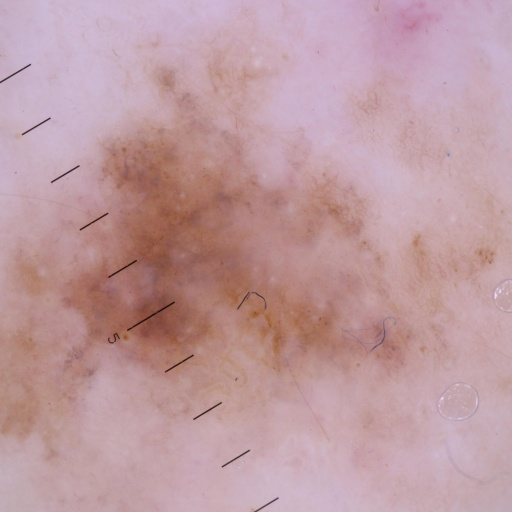
\includegraphics[height = 50mm, width=50mm]{imgs/mal_ex1.jpg}}\hspace{0.5em}
\subcaptionbox*{}{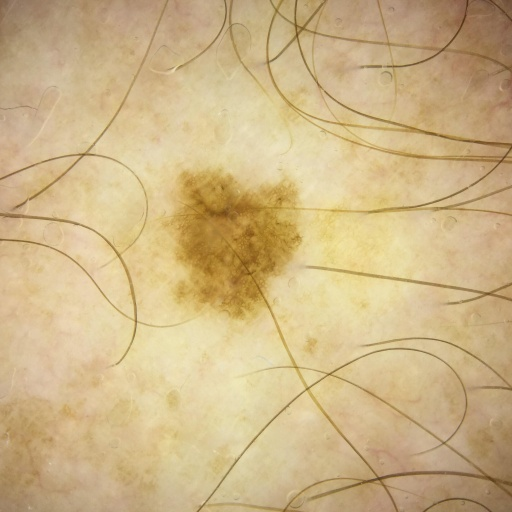
\includegraphics[height = 50mm, width=50mm]{imgs/mal_ex2.jpg}}\hspace{0.5em}
\subcaptionbox*{}{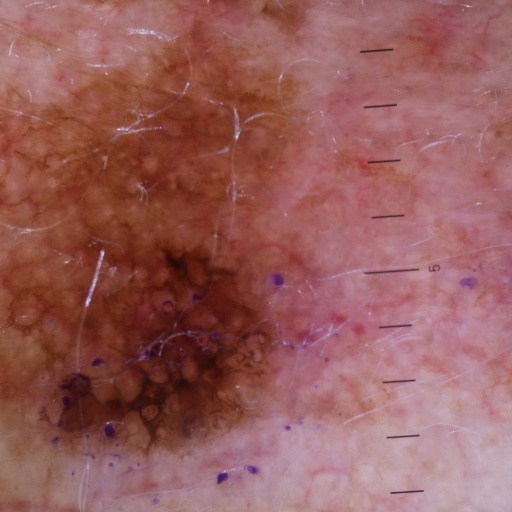
\includegraphics[height = 50mm, width=50mm]{imgs/mal_ex3.jpg}}
\hspace*{\fill}
\label{fig:mel_examples}
\vspace{-1cm}
\caption{Examples of Malignant Skin Lesions (\cite{ISIC})}
\end{figure}

\begin{figure}[hbt!]
\hspace*{\fill}
\centering
\subcaptionbox*{}{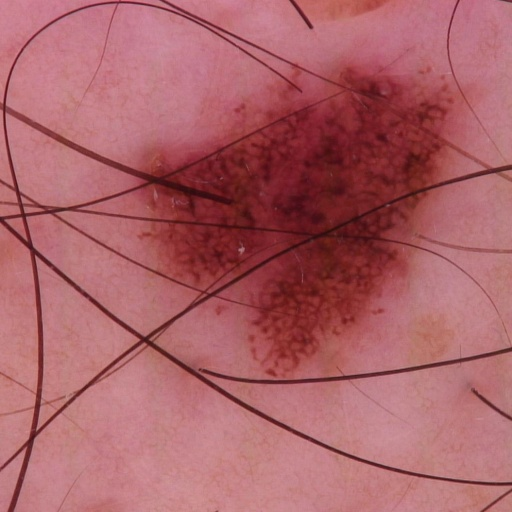
\includegraphics[height = 50mm, width=50mm]{imgs/ben_ex1.jpg}}\hspace{0.5em}
\subcaptionbox*{}{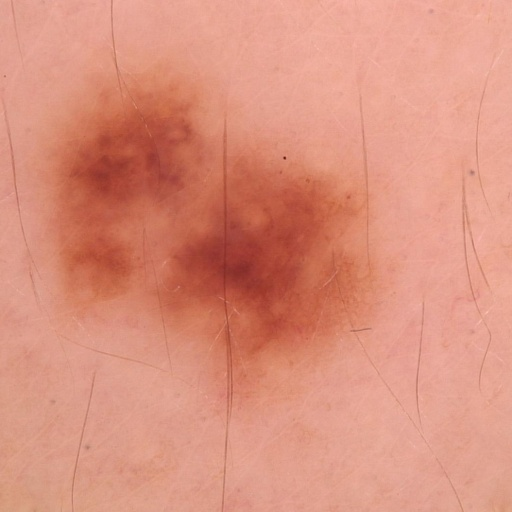
\includegraphics[height = 50mm, width=50mm]{imgs/ben_ex2.jpg}}\hspace{0.5em}
\subcaptionbox*{}{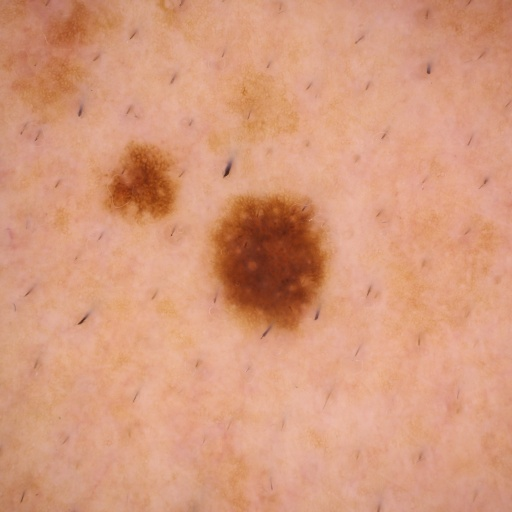
\includegraphics[height = 50mm, width=50mm]{imgs/ben_ex3.jpg}}
\hspace*{\fill}
\label{fig:ben_examples}
\vspace{-1cm}
\caption{Examples of Benign Skin Lesions (\cite{ISIC})}
\end{figure}


We also visually compared a random collection of images flagged as malignant with another random collection of images flagged as benign. The objective here was to see if our ``untrained'' eyes could easily classify the skin lesions as malignant or benign. We can see from Figures 2.1-2.2 that without proper training and education, it is very difficult to determine whether or not a skin lesion is actually malignant. Even with the proper training, it can still be difficult to accurately determine if melanoma is present. According to the Skin Cancer Foundation, features such as asymmetrical shapes, irregular borders, uneven distribution of color, and large relative size may indicate the presence of melanoma (or other skin cancers) \cite{SCF}. Ideally, our convolutional neural networks will pick up on these characteristics while training.

\subsection{Patient-Level Features}

In this section, we explore the one-way frequency tables for the approximate ages, patient sex, and the locations of the imaged lesions. Then we explore the two-way frequency tables for each of these variables with the response variable (malignant or benign).

\subsubsection*{Patient Age}

We can see from the histogram of approximate ages in Figure 2.3(a) that most of the patients in this data are in their 40's, 50's, and 60's. The box-plot in Figure 2.3(b) indicates that older patients are generally associated with a larger number of malignant skin lesions. In fact, we conducted a two-sample $t$-test (one-sided) to compare the mean age between the two groups. The $t$-test reported a p-value very close to 0, so we reject the hypothesis that the true group means are the same, and conclude that the mean age of patients with malignant skin lesions is significantly larger than the mean age of patients with benign skin lesions.

\begin{figure}[hbt!]
\hspace*{\fill}
\centering
\subcaptionbox{}{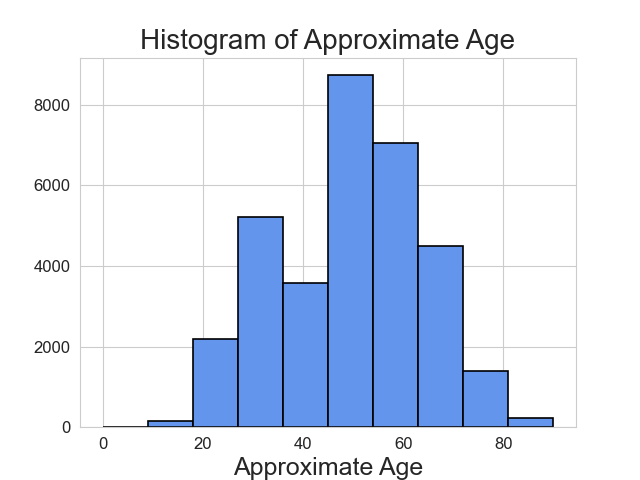
\includegraphics[height = 60mm, width=80mm]{imgs/age.png}}\hspace{0.5em}
\subcaptionbox{}{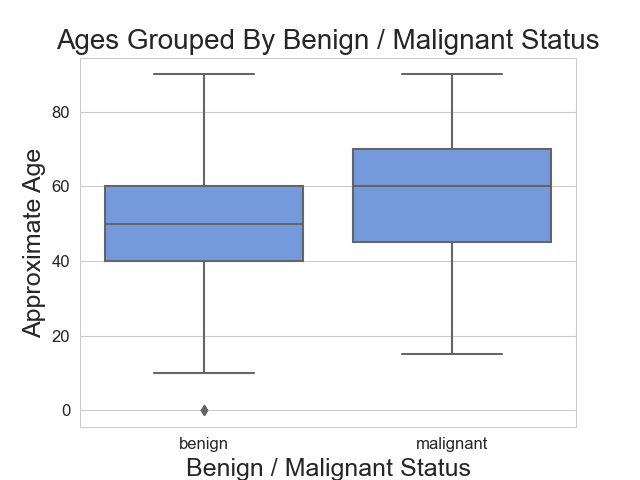
\includegraphics[height = 60mm, width=80mm]{imgs/age_2way.png}}
\hspace*{\fill}
\label{fig:age_eda}
\vspace{0cm}
\caption{Histogram and Box-Plot For Approximate Age}
\end{figure}

\subsubsection*{Patient Sex}

We can see from the frequencies shown in Figure 2.4(a) that there are a similar number of males and females in this dataset, with only about one thousand more males. The two-way contingency table between the response variable and patient sex is also shown in Figure 2.4(b). We can see that the malignant cases have a much larger proportion of males than the benign cases do. In fact, the $\chi^2$-test of independence reported a p-value very close to 0. Therefore, we reject the hypothesis that patient sex and the presence of melanoma are independent, and conclude that there is a relationship between the two variables.

\begin{figure}[hbt!]
    \hspace*{\fill}
    \centering
    \subcaptionbox{}{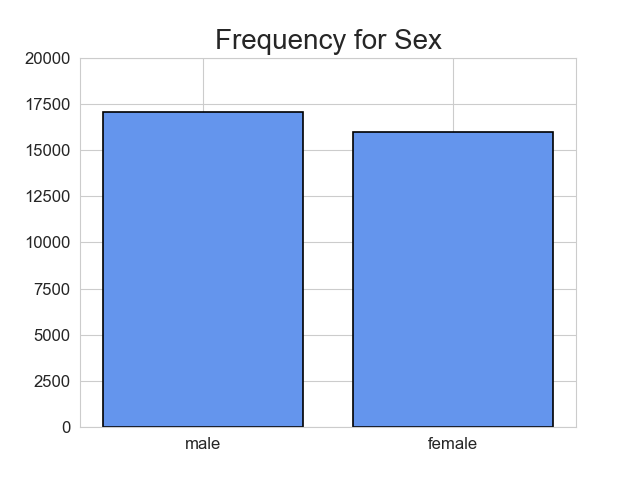
\includegraphics[height = 60mm, width=80mm]{imgs/sex.png}}\hspace{1em}
    \subcaptionbox{}{\vspace{17mm} \footnotesize \begin{tabular}{| c || c | c |} 
        \hline
        & \textbf{Benign} & \textbf{Malignant} \\ 
        \hline
        \hline
        \textbf{Female} & 15761 & 220\\
        \hline
        \textbf{Male} & 16716 & 364\\
        \hline  
        \end{tabular}}
    \hspace*{\fill}
    \label{fig:sex_eda_tab}
    \vspace{0cm}
    \caption{Frequency Plot and Two-way Contingency Table for Patient Sex}
    \end{figure}

\subsubsection*{Skin Lesion Location}

There were 6 categories for the general skin lesion location: oral/genital, palms/soles, head/neck, upper extremity, lower extremity, and torso. Figure 2.5(a) presents the associated frequencies within our dataset. None of the general locations have a similar number of counts, and almost half of the skin lesions come from the torso region.

\begin{figure}[hbt!]
    \hspace*{\fill}
    \centering
    \subcaptionbox{}{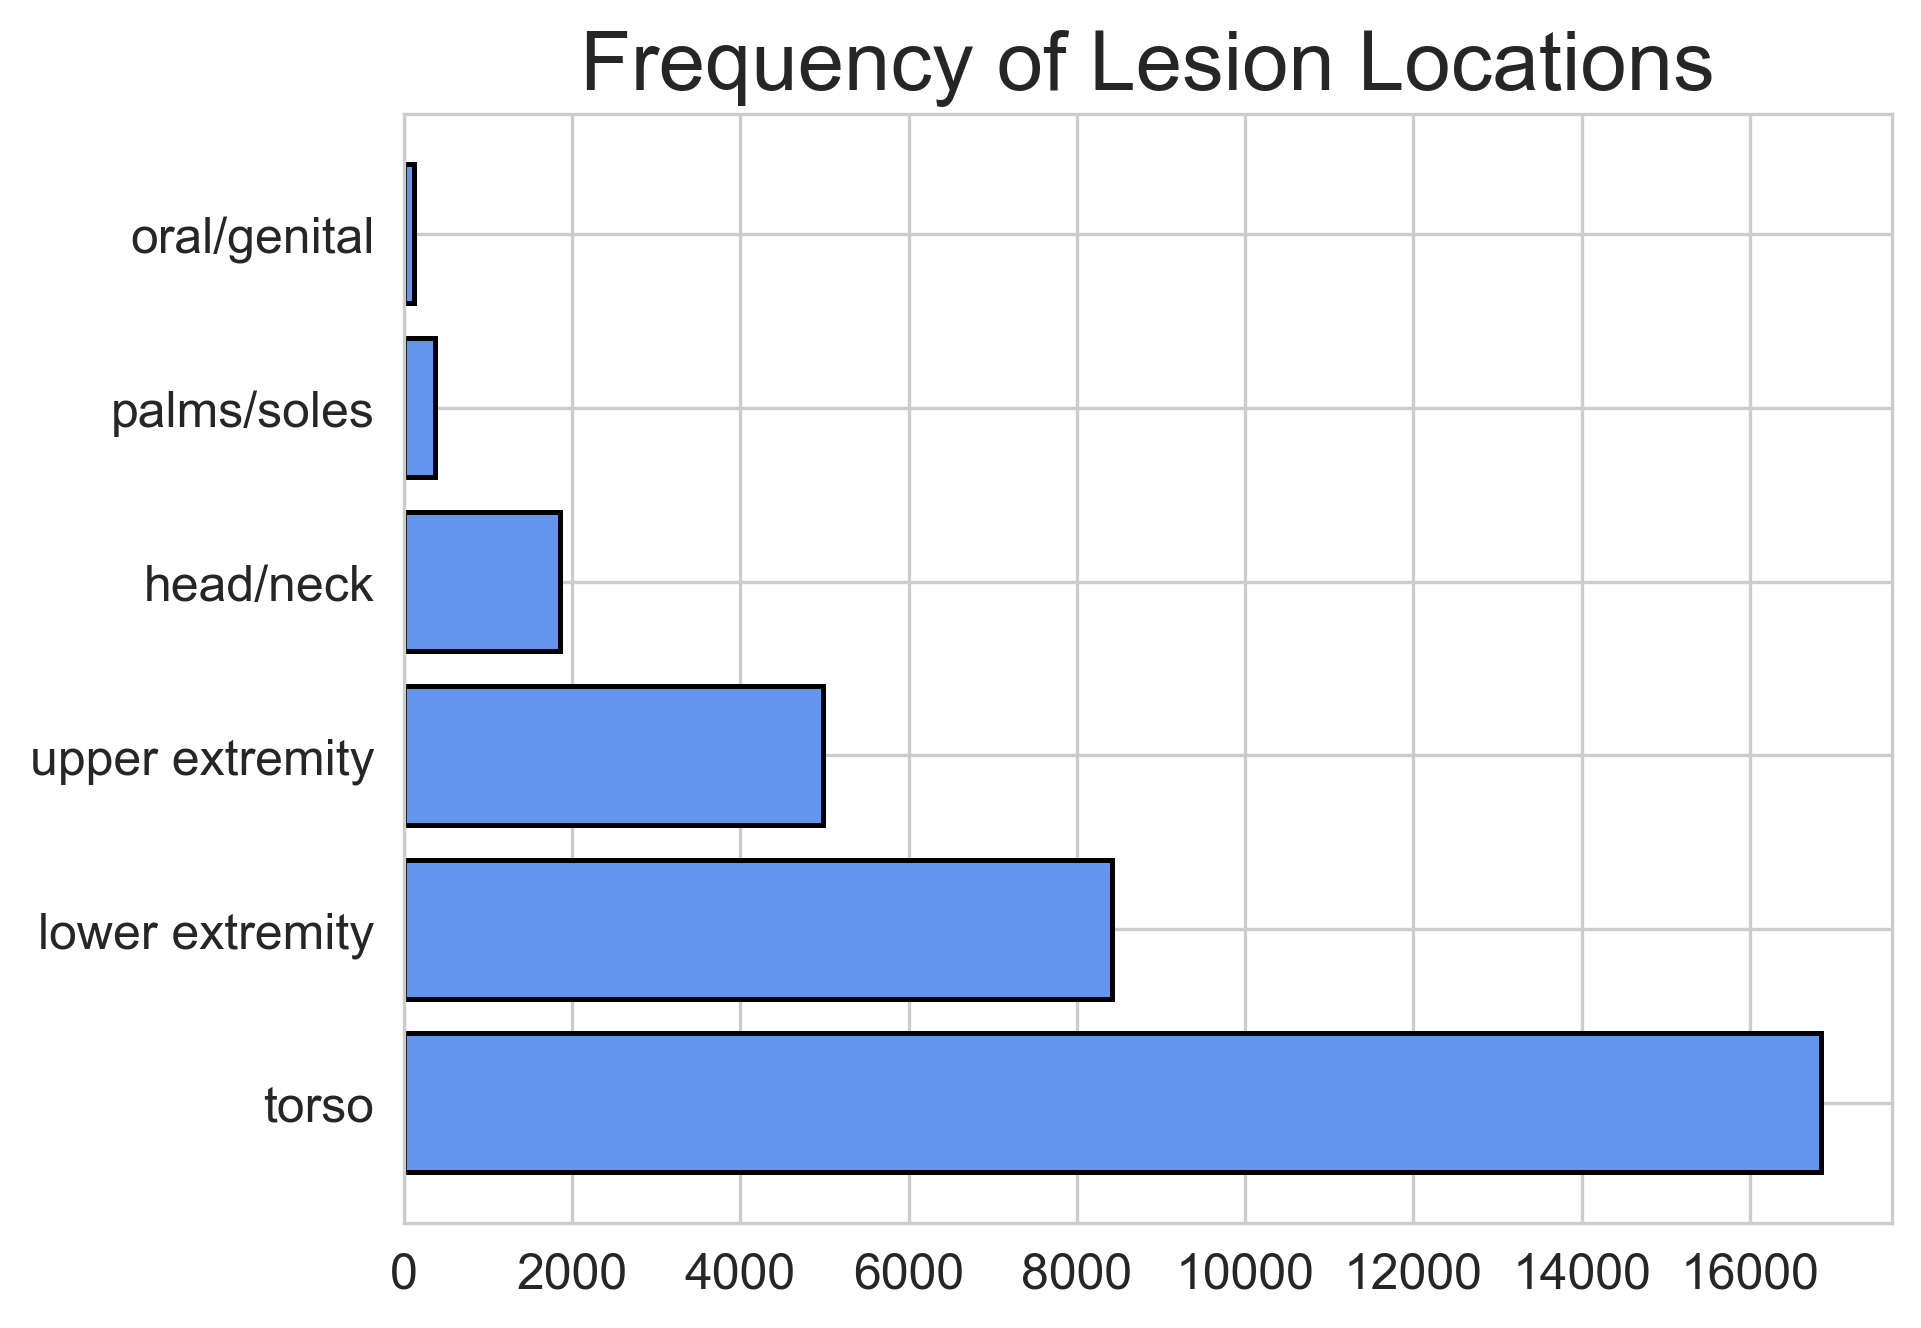
\includegraphics[height = 60mm, width=80mm]{imgs/site.png}}\hspace{1em}
    \subcaptionbox{}{\vspace{5mm} \footnotesize \begin{tabular}{| c || c | c |} 
        \hline
        & \textbf{Benign} & \textbf{Malignant} \\ 
        \hline
        \hline
        \textbf{Head/Neck} & 1781 & 74\\
        \hline
        \textbf{Lower Extremity} & 8293 & 124\\
        \hline  
        \textbf{Oral/Genital} & 120 & 4\\
        \hline
        \textbf{Palms/Soles} & 370 & 5\\
        \hline  
        \textbf{Torso} & 16588 & 257\\
        \hline
        \textbf{Upper Extremity} & 4872 & 111\\
        \hline  
        \end{tabular}}
    \hspace*{\fill}
    \label{fig:loc_eda_tab}
    \vspace{0cm}
    \caption{Frequency Plot and Two-way Contingency Table for Skin Lesion Location}
    \end{figure} 

\ 

We also present the two-way contingency table between the response variable and lesion location in Figure 2.5(b). While it is somewhat difficult to tell, there does appear to be some differences in the balance between benign and malignant cases when conditioned on the skin lesion location. In this case, the $\chi^2$-test of independence also reported a p-value very close to 0, indicating that there is a relationship between the location of the skin lesion and the presence of melanoma.


\chapter{Methodology}

In this section, we describe the methods and models used to best predict the presence of melanoma. As mentioned above, we used deep convolutional neural networks to generate classifications. More specifically, the latest variant of the residual network, the ResNeSt, was used to assess whether or not its channel-wise attention architecture would find further success in melanoma detection. Additionally, we trained a smaller, more generic, convolutional neural network to compare the performance with the split-attention network. 

To make use of the additional metadata features within our dataset, we simultaneously trained a standard \textit{multi-layer perceptron} (MLP) with inputs from our patient-level features. Therefore, the deep convolutional networks were used to effectively extract the contextualized features from the skin lesion images while the multi-layer perceptron was used to extract any important patient-level information. The two networks were fused to each other prior to generating a final probability. Since the predicted probabilities are a result from two separate networks communicating with each other, this model may be described as a \textit{Multi-Network Ensemble}. For convenience, the baseline model using the generic convolutional neural network and the multi-layer perceptron was named ``Ensemble \#1'', while the model using the ResNeSt architecture and the multi-layer perceptron was named ``Ensemble \#2''.

\section{Training, Validation, and Testing Sets}

Before discussing the actual models used, we briefly discuss how the dataset was split and sampled for training, validating, and testing.

We first randomly split 80\% of the data into a training set and used the other random 20\% as the test set. The test set was
not used by any model during the training process. Additionally, we partitioned another 20\% of the training data into a validation set. Recall that our dataset is largely imbalanced. As shown in the Exploratory Data Analysis section, only about 2\% of the skin lesions from the dataset are flagged as malignant, while the remaining skin lesions are marked as benign. We confirmed that each split of the data had a similar sample proportion of about 2\% malignant skin lesions.

Since the response variable (malignant or benign) in the training data is heavily imbalanced, we used randomized oversampling of the malignant observations to combat any potential bias toward a ``benign'' classification. By oversampling, we hoped that the models would better detect when skin lesions were truly malignant. It is important to note that since oversampling was used, we considered a single epoch as when the entire \textit{oversampled} dataset was passed forward and backward through the network exactly once. Therefore, a single epoch will contain multiple repeated malignant skin lesion images.

Note that using standard $k$-fold cross validation would require a model to be trained $k$ times for each set of hyperparameters. Given the size of our data and our models, the time it would have taken to perform this procedure would have been impractical. Therefore, we used the independent validation set to tune each network's hyperparameters effectively. This method minimized overall training time, and produced optimal hyperparameters. Once the hyperparameters were obtained, we retrained the model on a new oversampled dataset made from combining the training and validation sets.

We tuned each model with the area under the \textit{Receiver Operating Characteristic} (ROC-AUC) as our performance
metric. The ROC-AUC was chosen over other metrics because it summarizes how well our model separates the two response
classes over \textit{all} possible thresholds (as opposed to a single predetermined threshold). 

\section{Image Augmentations}

\textit{Image augmentations} were used as a preprocessing step for each image before training. Some image augmentation methods are often used to alter the original images in the dataset to effectively create more ``unseen'' examples for the network to use while training. These techniques artificially extend the dataset by randomly providing alterations to existing data, and consequently reduces the chance of overfitting. Given the limited number of malignant examples in our data, this technique was very important to artificially extend our malignant skin lesion training images. In our networks, we randomly employed the following image augmentations (in this order) on our training data \cite{AUG}:

\begin{enumerate}
    \item \textbf{HueSaturationValue}: With probability $p=0.5$, we randomly changed the hue, saturation, and value of the input image. The shift in hue was between $(-5, 5)$, the shift in saturation was between $(-10, 10)$, and the shift in value was between $(-5, 5)$.
    \item \textbf{FancyPCA}: With probability $p=0.2$, we performed \textit{principal component analysis} on the set of RGB pixel values throughout the input image, then added multiples of the found principal components, with magnitudes proportional to the corresponding eigenvalues times a random variable drawn from $\alpha_1, \alpha_2, \alpha_3 \stackrel{i.i.d}{\sim} \mathcal{N}(0, 0.1)$.
    \item \textbf{VerticalFlip}: With probability $p=0.5$, we vertically flipped the input image. Note that vertically flipping the image should not change the true class of the skin lesion.
    \item \textbf{HorizontalFlip}: With probability $p=0.5$, we horizontally flipped the input image. Note that horizontally flipping the image should not change the true class of the skin lesion.
    \item \textbf{GaussNoise}: We applied Gaussian noise to the input image. We did not want to corrupt the image too much and/or too often, so we used a mean of $0$ and a variance between $(10, 50)$ with a low probability $p=0.2$.
    \item \textbf{ShiftScaleRotate}: With probability $p=0.5$, we randomly applied the following three affine transforms: translation, scaling, and rotation of the input image. The shift factor range for both height and width was set to $(-0.25, 0.25)$, the scaling factor range was set to $(-0.25, 0.25)$, and the rotation range was set from $-30$ degrees to $30$ degrees. 
    \item \textbf{RandomBrightnessContrast}: With probability $p=0.5$, we randomly modified the brightness and contrast of the input image. Since many of the images were already very dark, the factor range for changing brightness was set to $(0.9, 1.1)$. The factor range for changing contrast was also set to $(0.9, 1.1)$.
\end{enumerate}

Some image augmentation techniques are also used to make sure the images in the dataset work with our models, and may promote faster convergence. For instance, in addition to the above augmentations, we also randomly cropped each $512 \times 512$ image to a $416 \times 416$ image and normalized the pixel values to have a similar distribution. Although the randomness of the cropping does somewhat ``artificially'' extend our training set, the main point of cropping the images to $416 \times 416$ is because the ResNeSt network we used requires an input size of $416 \times 416$ pixels. The normalization of the pixel values will reduce the risk of exploding gradients, which has been shown to increase training time and generally slows down convergence. We normalized each channel using the associated sample means and sample standard deviations calculated from the \textit{ImageNet} database. The ImageNet database consists of millions of images and was designed for use in visual object recognition software research. Although we could have used the sample means and sample standard deviations from our own dataset, using the sample statistics from the ImageNet database is common practice and was recommended by the authors of the ResNeSt network \cite{pt_resnest}.

We should note that most of the above image augmentations were only used on the training set. The validation and testing sets only center cropped the images to $416 \times 416$ and normalized the pixels to work with the trained networks.

\section{Network Architectures \& Training}

In this section, we provide an overview of the foundational neural network architectures, and we briefly discuss how our networks were trained \cite{MLnote}. We also introduce a few of the techniques we employed to combat overfitting.

\subsection{Multi-Layer Perceptrons}

As illustrated in Figure 3.1, a standard multi-layer perceptron (MLP) model consists of an input layer and an output layer, with at least one hidden layer in between. 


\begin{figure}[h]
\centering
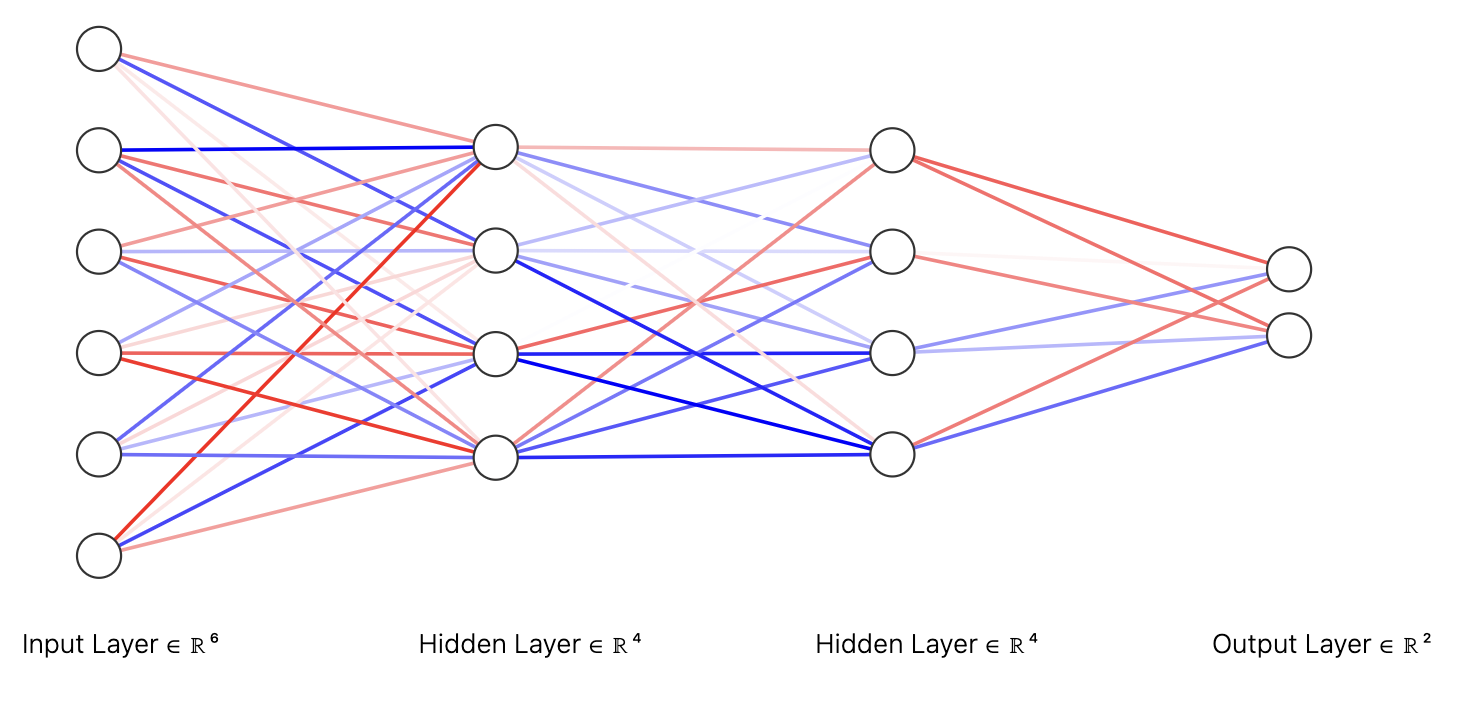
\includegraphics[height = 80mm, width=145mm]{imgs/ffn.png}
\caption{Multi-Layer Perceptron (Feed-Forward Network) Example}
\label{fig:ffn}
\end{figure}

The $l$th layer within the network may be represented by a vector, $\mathbf{h}^{(l)}$, which is obtained by applying a Sigmoid or ReLU transform to the product of the $(l-1)$th layer and a weight matrix, $\mathbf{W}^{(l)}$, plus a bias vector, $\mathbf{b}^{(l)}$. That is, the general MLP has the following recursive structure, $$\mathbf{h}^{(l)} = f_l(\mathbf{s}^{(l)})$$
$$\mathbf{s}^{(l)} = \mathbf{W}^{(l)}\mathbf{h}^{(l-1)} + \mathbf{b}^{(l)}$$ for $l=1, 2, ..., K$. Here, $K$ is the number of layers in the network, $\mathbf{h}^{(0)}$ represents our input features $\mathbf{X}$, $\mathbf{h}^{(K)}$ represents the outputted probabilities used to make the final classification for our response, $\mathbf{Y}$, and $f_l$ is an element-wise transformation. Following industry standards, our networks used the ReLU activation function for all hidden layers such that $f_l(s^{(l)}_j) = \text{ReLU}(s^{(l)}_j) = \max(0, s^{(l)}_j)$ for $l=1, 2, ..., K-1$ and the softmax function (or sigmoid function if $s^{(K)} \in \mathbb{R}$) for the output layer such that the $j$th outputted probability is:

$$\hat{p}_j = f_K(\mathbf{s}^{(K)})_j = \frac{e^{s^{(K)}_j}}{\sum_i e^{s^{(K)}_i}} \in (0, 1)$$

\subsection{Methods of Learning}

In general, neural networks are trained by minimizing a chosen loss function $L$, with some form of gradient descent. The gradients for each layer's weights $\mathbf{W}_l$ and biases $\mathbf{b}_l$ are calculated using \textit{back-propogation}. Back-propogation is the process of applying chain rule as many times as necessary to obtain the gradient for a specified weight or bias. Given the network structure described above, the following relationships between gradients can be easily shown with chain rule:
$$\frac{\partial L}{\partial \mathbf{h}^{(l-1) \text{ }T}} = \frac{\partial L}{\partial \mathbf{h}^{(l) \text{ }T}} f'_{l} \mathbf{W}^{(l)} \text{,\quad \quad} \frac{\partial L}{\partial \mathbf{W}^{(l)}} = f'_{l} \frac{\partial L}{\partial \mathbf{h}^{(l)}}\mathbf{h}^{(l-1) \text{ }T} \text{,\quad \quad} \frac{\partial L}{\partial \mathbf{b}^{(l)}} = f'_{l} \frac{\partial L}{\partial \mathbf{h}^{(l)}}$$ where $f'_{l} = \text{diag}(f'(s^{(l)}_{j})  \text{; for } j = 1, 2, ... d)$.


For notational convenience, we can represent our training data as $(\mathbf{x}_i, y_i)$ for $i = 1, 2, ..., N$ and our network parameters as $\theta = (\mathbf{W}_l, \mathbf{b}_l  \text{; for } l = 1, 2, ... K)$. Since we have a binary response variable (the skin lesion is either malignant or benign), we trained our networks using the \textit{Binary Cross-Entropy} loss function defined as: 

$$L(y_i, \mathbf{x}_i; \theta) = - \left[ y_i\log(\hat{p}(\mathbf{x}_i)) + (1 - y_i)\log(1 - \hat{p}(\mathbf{x}_i)) \right]$$ 

As mentioned above, this loss function is used to train the network's parameters with a form of gradient descent. With $\mathcal{L}(\theta) = \frac{1}{N} \sum_{i=1}^{N} L(y_i, \mathbf{x}_i; \theta)$ as the averaged loss over the entire training set, the standard gradient descent algorithm has the following form: $$\theta_{t+1} = \theta_{t} - \eta_t \mathcal{L}'(\theta_t)$$ where $\mathcal{L}'(\theta_t)$ is the gradient and $\eta_t$ is the learning rate ($\eta_t \propto \frac{1}{t}$). The general idea of this algorithm is to pass the training data through the network (known as the \textit{forward pass}), use these predictions with the loss function to calculate the resulting gradients (known as the \textit{back-propagation pass}), then use these gradients to update the parameters as shown above. Although not always guaranteed, this algorithm should find the weights and biases $\theta$ that minimize the binary cross-entropy loss function. 

Practically speaking, computing $\mathcal{L}'(\theta_t) = \frac{1}{N} \sum_{i=1}^{N} L'(y_i, \mathbf{x}_i; \theta_t)$ would be far too time-consuming with a massive training set and a large number of parameters. Instead, we use a randomly selected mini-batch of size $m$ to replace $\mathcal{L}(\theta_t)$ with its estimate: $$\hat{\mathcal{L}}(\theta_t) = \frac{1}{m} \sum_{j=1}^{m} L(y_j, \mathbf{x}_j; \theta_t)$$ when updating the parameters. Using $\hat{\mathcal{L}}'(\theta_t)$ in the gradient descent algorithm is known as \textit{Stochastic Gradient Descent}. It reduces the computation cost at each iteration, and will ideally lead to similar results (assuming a true randomly sampled batch and a large enough $m$). One \textit{epoch} occurs after the entire training set has been passed though the network exactly once. Therefore, with stochastic gradient descent, a single epoch occurs after about $t=\frac{N}{m}$ updates to the network parameters.

At each iteration, the stochastic gradient descent algorithm described above will always update the parameters in the direction of the steepest downward direction. However, this direction may not always be the ideal choice. Depending on the level of noise and the loss function itself, it may be valuable to consider characteristics such as the momentum of the movement and the unevenness of the individual parameter components. The \textit{Adam} optimizer modifies the stochastic gradient descent algorithm by considering the direction of the momentum and includes an adaptive mechanism to reduce the effects of extremely uneven gradient components. At the $t$th iteration, momentum is characterized by: $$\nu_t = \frac{1}{(1-\gamma)} \left[ \gamma \nu_{t-1} + (1-\gamma)\hat{\mathcal{L}}(\theta_t) \right]$$ and the mechanism used to adjust the uneven components is: $$G_t = \frac{1}{(1-\beta)} \left[ \beta G_{t-1} + (1-\beta)\hat{\mathcal{L}}(\theta_t) \odot \hat{\mathcal{L}}(\theta_t)\right]$$ where $\gamma, \beta \in \mathbb{R}$ are tunable hyperparameters that are generally set such that $\gamma, \beta \in (0.9, 1)$, and the $\odot$ operator represents element-wise multiplication. Consequently, we used these mechanisms to update the network parameters such that: $$\theta_{t+1} = \theta_{t} - \eta_t \frac{\nu_t}{\sqrt{G_t + \varepsilon}}$$ Here $\varepsilon>0$ is a very small constant to avoid division by 0. Note that the general structure of the parameter update still remains similar to stochastic gradient descent, however, each update also considers the momentum from the previous updates and the variation in the gradient components.

Our melanoma detection networks were trained using this Adam optimizer with $\gamma$ and $\beta$ fixed at $0.9$ and $0.999$, respectively. Each mini-batch consisted of $m=20$ training examples.  Throughout training, the initial learning rate $\eta_t$ was tuned using our validation set, however, we customized our networks to tune different learning rates for different branches. That is, the weights and biases from the convolutional network within our ensemble had a \textit{separately tuned} learning rate from the other parts of our ensemble. This is discussed with more detail in Section 3.3.8. Additionally, all learning rates were scheduled to decay by a multiplicative factor of $\gamma_{\text{LR}}$ after each epoch to avoid potential oscillations about the minimum and to promote a quicker convergence.

\subsection{Preventing Overfitting}

Given the large number of parameters, neural networks will often overfit the training data if precautions are not taken. Overfitting occurs when the network effectively fits the random noise within the training data, and lacks the ability to generalize to unseen data. Figure 3.2 shows the general trend of the training loss and the validation loss as we train our network. The idea is that if we train our model for too long, it will overfit the training data and the predictive performance will be suboptimal for the validation (or test) dataset. 

\begin{figure}[h]
\centering
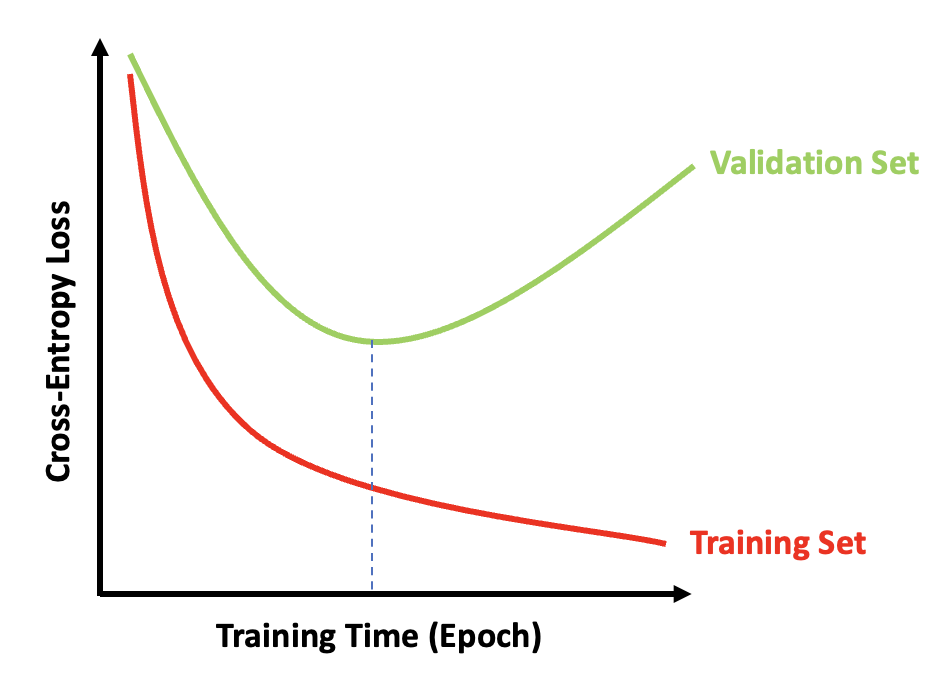
\includegraphics[height = 75mm, width=110mm]{imgs/overfitting.png}
\caption{Overfitting Illustration}
\label{fig:ovfit}
\end{figure}

To prevent our networks from overfitting the training data, we used the validation set to obtain performance updates throughout training, and stopped the training once the validation performance began declining. The goal was to use the parameters that correspond to the minimum validation loss, or maximum validation performance. The vertical dotted line in Figure 3.2 indicates this ideal stopping point. 

In our case, we generated a validation performance update after each half-epoch of training. At each half-epoch, we calculated the ROC-AUC score and the binary cross-entropy loss for the validation data, and discontinued the training if these scores dropped or stayed the same in back-to-back performance updates.

There are other methods to help prevent overfitting from occurring. For instance, image augmentation may help prevent the chances of overfitting by artificially increasing the size of the training set. We also used \textit{L2-regularization} for our network parameters. This form of regularization within neural networks is also referred to as \textit{weight-decay}. In general, L2-regularization adds a penalty term, $J(\theta)$, to the loss function such that the new goal would be to minimize $\mathcal{L}(\theta) + \lambda J(\theta)$ where: $$J(\theta) = \sum_{l, j, k} {W^{(l)}_{j, k}}^2 + \sum_{l, k} {b^{(l)}_{k}}^2$$ and $\lambda > 0$ is a hyperparameter that we tune while training \cite{ESL}. 

In addition to regularization, we also included \textit{dropout} layers to prevent overfitting. Dropout layers refer to the dropping of a random selection of nodes within a specified layer of the network. All of the connections associated with a dropped node are consequently removed, and the ``new'' network is made up of a subset of the original nodes and connections. Dropout can be thought of as another form of regularization because it effectively prevents neurons in a layer from heavily depending on a specific input. Therefore, preventing the overreliance of a single input should reduce the variance of the network parameters. 

Dropout regularization was frequently used throughout our ensemble's networks with $p = 0.2$, meaning that a random 20\% of the layer's corresponding neurons were masked throughout training. 


\subsection{Batch Normalization}

When training the neural network with back-propagation, the distribution of each layer's inputs, $\mathbf{h}^{(l)}$ for $l=1, 2, ..., K$, may often change because the parameters of previous layers ($< l$) are also changing with every mini-batch update. This phenomenon is known as \textit{internal covariate shift}, and it has been shown to drastically slow training time down \cite{BatchNorm}. In our networks, we stabilized the distributions of each layer's inputs, $\mathbf{h}^{(l)}$ for $l=1, 2, ..., K$, using \textit{batch normalization} \cite{BatchNorm}. Therefore, between $\mathbf h^{(l)}$ and $\mathbf h^{(l+1)}$, we added a batch normalization layer that transforms $\mathbf{h}^{(l)}$ to $\tilde{\mathbf{h}}^{(l)}$ to help stabilize its distribution and reduce the internal covariate shift. Then, $\tilde{\mathbf{h}}^{(l)}$ is fed into the next layer for the computation of $\mathbf{h}^{(l+1)}$. 

More formally, consider a mini-batch size of $m$, and a layer input $\mathbf{h}^{(l)} = (h^{(l)}_1, ..., h^{(l)}_d)^T \in \mathbb{R}^d$. Batch normalization is applied to each element of $\mathbf{h}^{(l)}$ independently, so for each $k \in \{1, 2, ..., d \}$, we have exactly $m$ values of this activation from the mini-batch. For simplicity, we denote the $i$th value from the $k$th activation by $x_{i,k}$ for $i \in \{1, 2, ..., m \}$ and $k \in \{1, 2, ..., d \}$. The batch normalization layer computes $$\mu_k = \sum_{i=1}^{m} x_{i, k} \text{, \quad} \sigma_k = \frac{1}{m} \sum_{i=1}^{m} (x_{i, k} - \mu_k)^2 \text{, \quad} \hat{x}_{i,k} = \frac{x_{i,k} - \mu_k}{\sigma_k} \text{, \quad} y_{i, k} = \beta + \gamma \hat{x}_{i,k}$$ where $\beta$ and $\gamma$ are learned while training. Here, $y_{i, k}$ represents the $i$th value (from the mini-batch) for the $k$th activation of the batch normalized layer, $\tilde{\mathbf{h}}^{(l)}$, where $i \in \{1, 2, ..., m \}$ and $k \in \{1, 2, ..., d \}$.

These batch normalization transformations were used after most of the convolutional and linear layers within our ensemble of networks. Although no tuning was necessary for this technique, we found that the inclusion of batch normalization layers significantly sped up training time.


\subsection{Convolutional Neural Networks}

The convolutional neural network (CNN) structure is often used for computer vision objectives. In general, a CNN is made up by a series of convolutional layers that filter down the training images to a single ``thought'' vector. This ``thought'' vector is usually a large linear layer with many nodes/elements that represents the extracted features from the images. The final ``thought'' vector is then followed by a series of fully-connected linear layers as if it were a standard multi-layer perceptron. We can think of the ``thought'' vector as a characterization of its associated image. Figure 3.3 illustrates the general idea. Through a variety of transformations and subsampling (or pooling) techniques, the original image is filtered down into a longer linear layer that is ultimately used as input for another feed-forward network.

\begin{figure}[h]
\centering
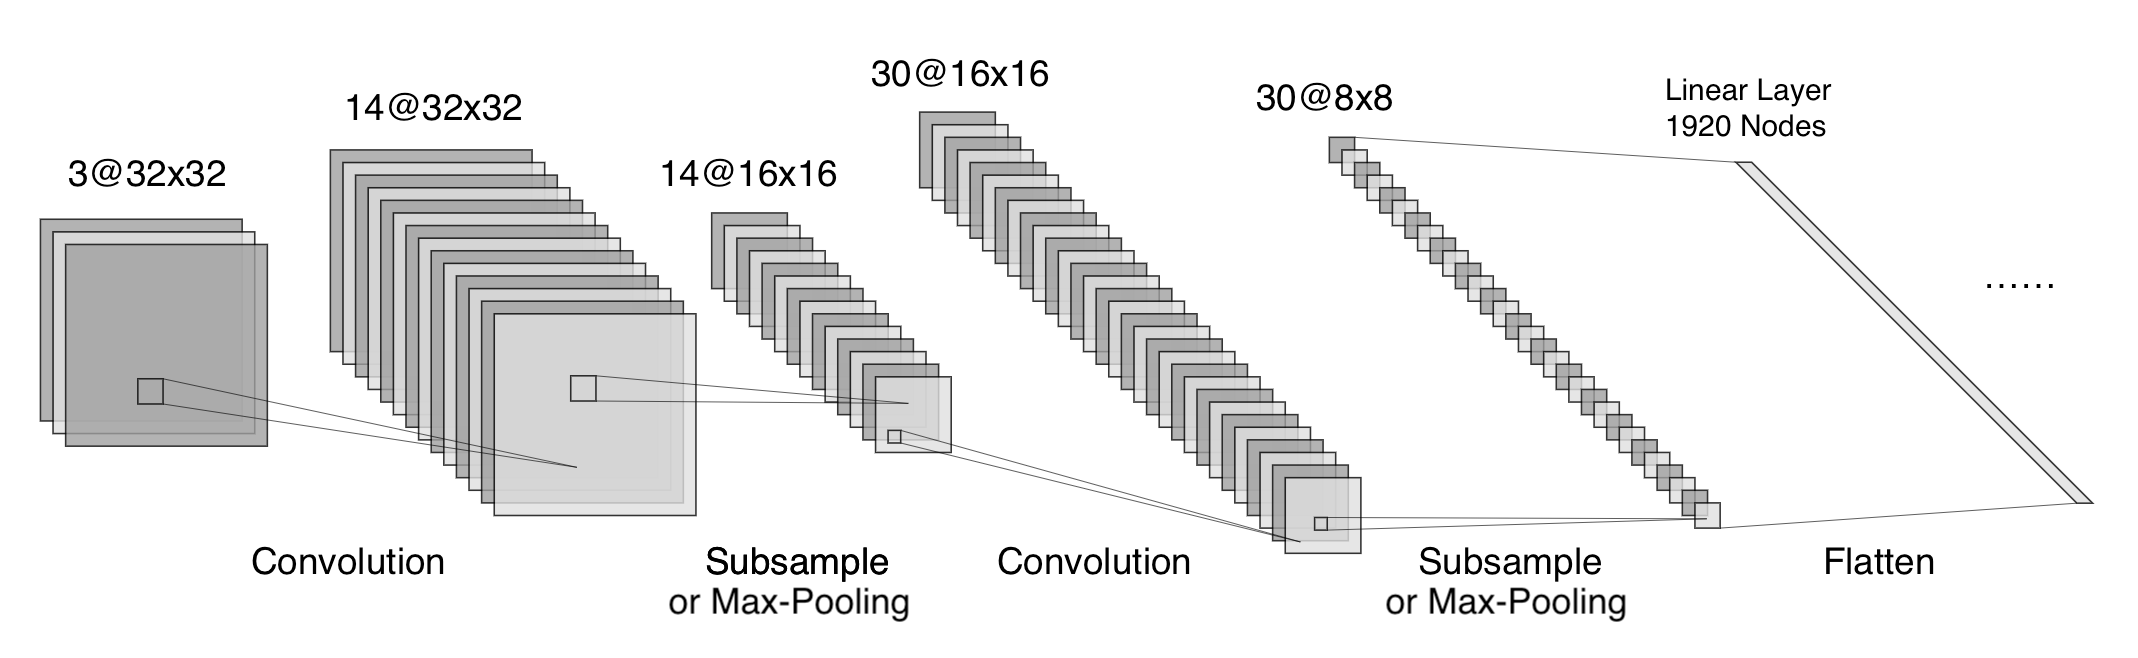
\includegraphics[height = 60mm, width=160mm]{imgs/cnn_s1.png}
\caption{Convolutional Neural Network Basic Structure}
\label{fig:cnn1}
\end{figure}

Each convolutional layer $\mathbf{h}^{(l)}$ is organized as a series of channels, where each channel is obtained by a kernel, $\mathbf{W}_{i, j}$, operating on the previous layer's $\mathbf{h}^{(l-1)}$, which was also organized as a series of channels.  Each kernel operation is a locally weighted sum of the values within each channel. That is, when there are multiple channels, this weighted sum is over the multiple channels. Once the weighted summations have been performed, a bias term is generally added, and a non-linear transformation, such as the ReLU activation function, is applied to the result. For example, consider Figure 3.3. The first layer, $\mathbf{h}^{(0)}$ is the input image with 3 channels (which correspond to red, green, and blue), and after applying the kernel operations with the bias term and ReLU transformation, the subsequent layer, $\mathbf{h}^{(1)}$, increases to 14 channels. 

We can also present the operations of a convolutional layer more formally. Let $\mathbf{x}_{i j} \in \mathbb{R}^{C_{l-1}}$ represent the vector of values at the $(i, j)$th coordinate for each of the $C_{l-1}$ channels in the $(l-1)$th layer, and let $\mathbf{y}_{i j} \in \mathbb{R}^{C_{l}}$ represent the vector of values at the $(i, j)$th coordinate for each of the $C_{l}$ channels in the $l$th layer. The kernel operation is equivalent to the following linear transformation: $$\tilde{\mathbf{x}}_{i j} = \sum_{\Delta i = -k_1}^{k_1} \sum_{\Delta j = -k_2}^{k_2} \mathbf{W}_{\Delta i \text{, } \Delta j} \text{ } \mathbf{x}_{i+\Delta i \text{, } j+\Delta j}$$ where $\mathbf{W}_{\Delta i \text{, } \Delta j} \in \mathbb{R}^{C^{l} \times C^{l-1}}$ is learned and the kernel dimensions are fixed at $2k_1 \times 2k_2$. As mentioned above, the bias term, $\mathbf{b}_{l}$, is added and the ReLU transformation is applied such that: $$\mathbf{y}_{i j} = \text{ReLU}(\tilde{\mathbf{x}}_{i j} + \mathbf{b}_{l})$$ where $\mathbf{b}_{l}$ is learned and the ReLU transformation is applied element-wise.

For each convolutional layer, a method of \textit{pooling} or \textit{subsampling} is generally done after the above transformations are performed. Pooling and subsampling methods are performed to effectively downsample the output of the convolutional layer along its spatial dimensions. That is, the size of each channel is reduced. While the convolutional operations are generally meant to increase the number of channels, the pooling or subsampling methods are applied to decrease the height and width of each channel. The primary goal of pooling and subsampling is to reduce the total number of parameters within the network. In addition, this may reduce the chance of overfitting to our training data and will significantly decrease training time.

\subsection{Ensemble \#1}

As mentioned previously, we trained a total of two multi-network ensembles. The first ensemble includes a standard CNN for the image data and a multi-layer perceptron for the patient-level metadata, while the second ensemble includes a ResNeSt network for the image data and a similar multi-layer perceptron for the patient-level metadata. Ensemble \#1 was simply used as a model to compare with Ensemble \#2. It can be thought of as a baseline model to assess the improvements provided by the split-attention network within the second ensemble. 

The CNN within the first ensemble contained a total of 6 convolutional layers. Each convolutional layer was immediately followed by batch normalization and downsampling. The convolutional layer within this ensemble exclusively applied \textit{max-pooling} as its downsampling method. For each channel, max-pooling simply replaces the value of each pixel by the maximum of a fixed-size patch surrounding the pixel. In this case, we decided to use max-pooling with a kernel size of $2 \times 2$ and a stride of 2 (the number of pixels between adjacent windows). Figure 3.4 demonstrates a simple example of how max-pooling is applied to the spatial data within each channel. 

\begin{figure}[h]
\centering
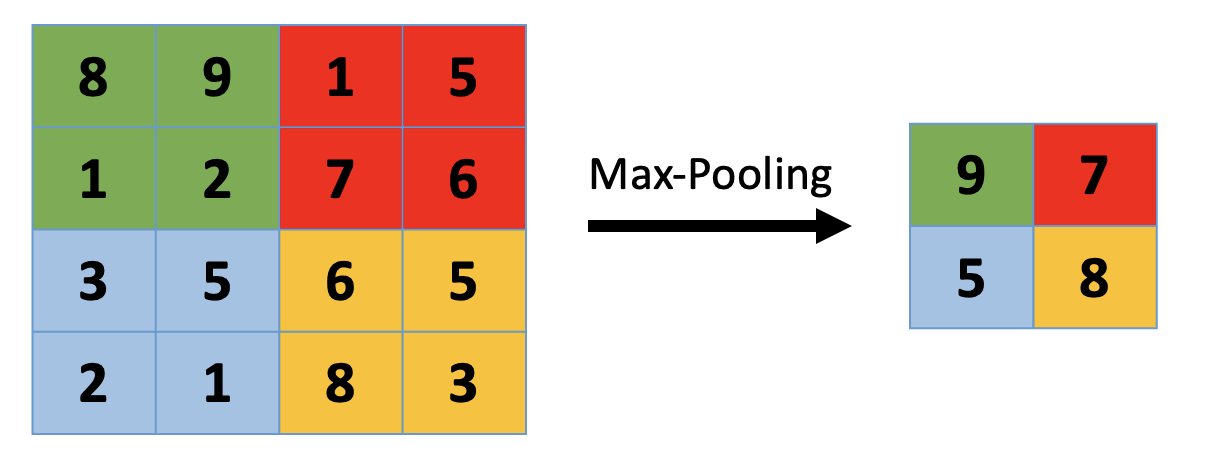
\includegraphics[height = 40mm, width= 100mm]{imgs/maxpool.png}
\caption{Max-Pooling Example with Filter-Size $2 \times 2$ and Stride 2}
\label{fig:maxpool}
\end{figure}

\begin{table}[h!]
\centering
\footnotesize 
\renewcommand{\arraystretch}{1.3}
\begin{tabular}{ c | c | c | c | c | c | c} 
\hline
\makecell{\textbf{Layer} \\ \textbf{Name}} & \makecell{\textbf{Output} \\ \textbf{Size}} & \textbf{Operation} & \makecell{\textbf{Output} \\ \textbf{Channel} \\ \textbf{Number}} & \textbf{Normalization} & \textbf{Activation} & \textbf{Pooling}\\ 
\hline
\hline
Conv1 & $253 \times 253$ & $7 \times 7$ & 6 & \makecell{Batch-Norm \\ (2D)} & ReLU & \makecell{Max-Pool \\ (2x2, stride=2)}\\
\hline
Conv2 & $124 \times 124$ & $7 \times 7$ & 15 & \makecell{Batch-Norm \\ (2D)} & ReLU & \makecell{Max-Pool \\ (2x2, stride=2)}\\
\hline
Conv3 & $59 \times 59$ & $7 \times 7$ & 30 & \makecell{Batch-Norm \\ (2D)} & ReLU & \makecell{Max-Pool \\ (2x2, stride=2)}\\
\hline
Conv4 & $26 \times 26$ & $5 \times 5$ & 60 & \makecell{Batch-Norm \\ (2D)} & ReLU & \makecell{Max-Pool \\ (2x2, stride=2)}\\
\hline
Conv5 & $11 \times 11$ & $5 \times 5$ & 80 & \makecell{Batch-Norm \\ (2D)} & ReLU & \makecell{Max-Pool \\ (2x2, stride=2)}\\
\hline
Conv6 & $3 \times 3$ & $3 \times 3$ & 100 & \makecell{Batch-Norm \\ (2D)} & ReLU & \makecell{Max-Pool \\ (2x2, stride=2)}\\
\hline
Linear1 & $1 \times 1$ & Fully Connected & 512 & \makecell{Batch-Norm \\ (1D)} & ReLU & N/A\\
\hline
Linear2 & $1 \times 1$ & Fully Connected & 512 & \makecell{Batch-Norm \\ (1D)} & ReLU & N/A\\
\hline  
\end{tabular}
\label{tab:CNN_arch}
\caption{CNN Architecture for Multi-Network Ensemble \#1}
\end{table}

After all 6 convolutional, normalization, and downsampling operations were applied, the original 3-channel image was filtered to a linear layer with exactly 900 nodes. As described above, this output should represent the high-level features within the images. We include two additional fully-connected layers, each with 512 nodes, in another attempt to learn any remaining non-linear combinations of these features. Note that all convolutional and linear layers associated with this network used the ReLU activation function. Table 3.1 includes the details regarding the specific architecture used for the CNN within Ensemble \#1.

In parallel to this convolutional network, a multi-layer perceptron takes the 7 patient-level features (after one-hot encoding) and connects it to a linear layer with 256 nodes. A batch normalization layer is also included, and dropout regularization with $p=0.2$ is used to prevent overfitting. Again, we note that the ReLU activation function was used for this multi-layer perceptron. 

\begin{figure}[h]
\centering
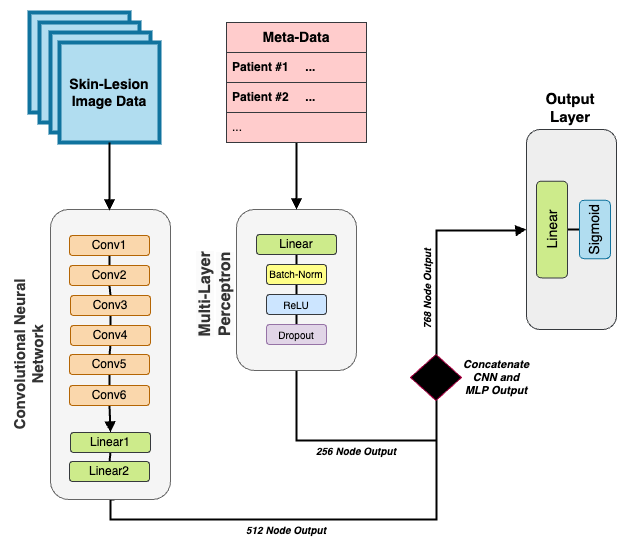
\includegraphics[height = 120mm, width= 140mm]{imgs/ens1_arch.png}
\caption{Multi-Network Ensemble \#1}
\label{fig:ens1_arch}
\end{figure}

Figure 3.5 illustrates how these two separate networks are effectively fused together for our first ensemble. The 512 node output corresponding to the image data is concatenated with the 256 node output corresponding to the patient-level metadata. This concatenated layer is then fed into the output layer, with a single node. Lastly, we applied the sigmoid function to the score of the output node to estimate the probability that the associated skin lesion is malignant. 

The framework of this first multi-network ensemble is very similar to the framework used in the second ensemble. In the next two sections, we introduce the ResNeSt network architecture and how it was leveraged to better extract the high-level features within the skin lesion images. Then, we provide the details regarding how it was implemented within Ensemble \#1.

\subsection{ResNeSt}

In 2015, Kaiming He introduced the residual neural network, or \textit{ResNet}, in the paper \textit{Deep Residual Learning for Image Recognition} \cite{resnet}. The ResNet model revolutionized the world of convolutional neural networks. Prior to the residual network architecture, deep neural networks faced the ``vanishing gradient'' difficulty while training. The ``vanishing gradient'' occurs when the gradients get very close to 0. In general, as the number of layers within a network increases, the gradients approach 0. Motivated by Taylor expansion, Kaiming introduced the technique known as the ``identity-skip connection'' or ``shortcut connection''. An identity-skip connection reduces the effect of gradient vanishing regardless of the number of layers within a network, and consequently allows for deeper networks to be built without negatively impacting training. 

In general, a residual network uses blocks of convolutional layers, in combination with an identity-skip connection (more formally known as \textit{identity mapping}). Each block of convolutional layers is referred to as a \textit{residual block}. Suppose $\mathbf{h}^{(l)}$ is the input to a residual block and $\mathbf{s}^{(l+1)}$ is the output of the residual block. If we denote the series of applied convolutional layers (weighted sums), batch normalizations, and ReLU activations by $\mathcal{F}$, then $\mathbf{s}^{(l+1)} = \mathbf{h}^{(l)} + \mathcal{F}(\mathbf{h}^{(l)})$. Figure 3.6 illustrates the idea of a residual block with an identity-skip connection. Note that the final ReLU activation is not applied until after the addition of the residual block output and the identity connection such that $\mathbf{h}^{(l+1)}$ can be found by applying the ReLU activation to $\mathbf{s}^{(l+1)}$. Additionally, if the dimensions of $\mathbf{h}^{(l)}$ and $\mathcal{F}(\mathbf{h}^{(l)})$ are not the same, a linear projection is used by the shortcut connections to match the dimensions.


\begin{figure}[h]
\centering
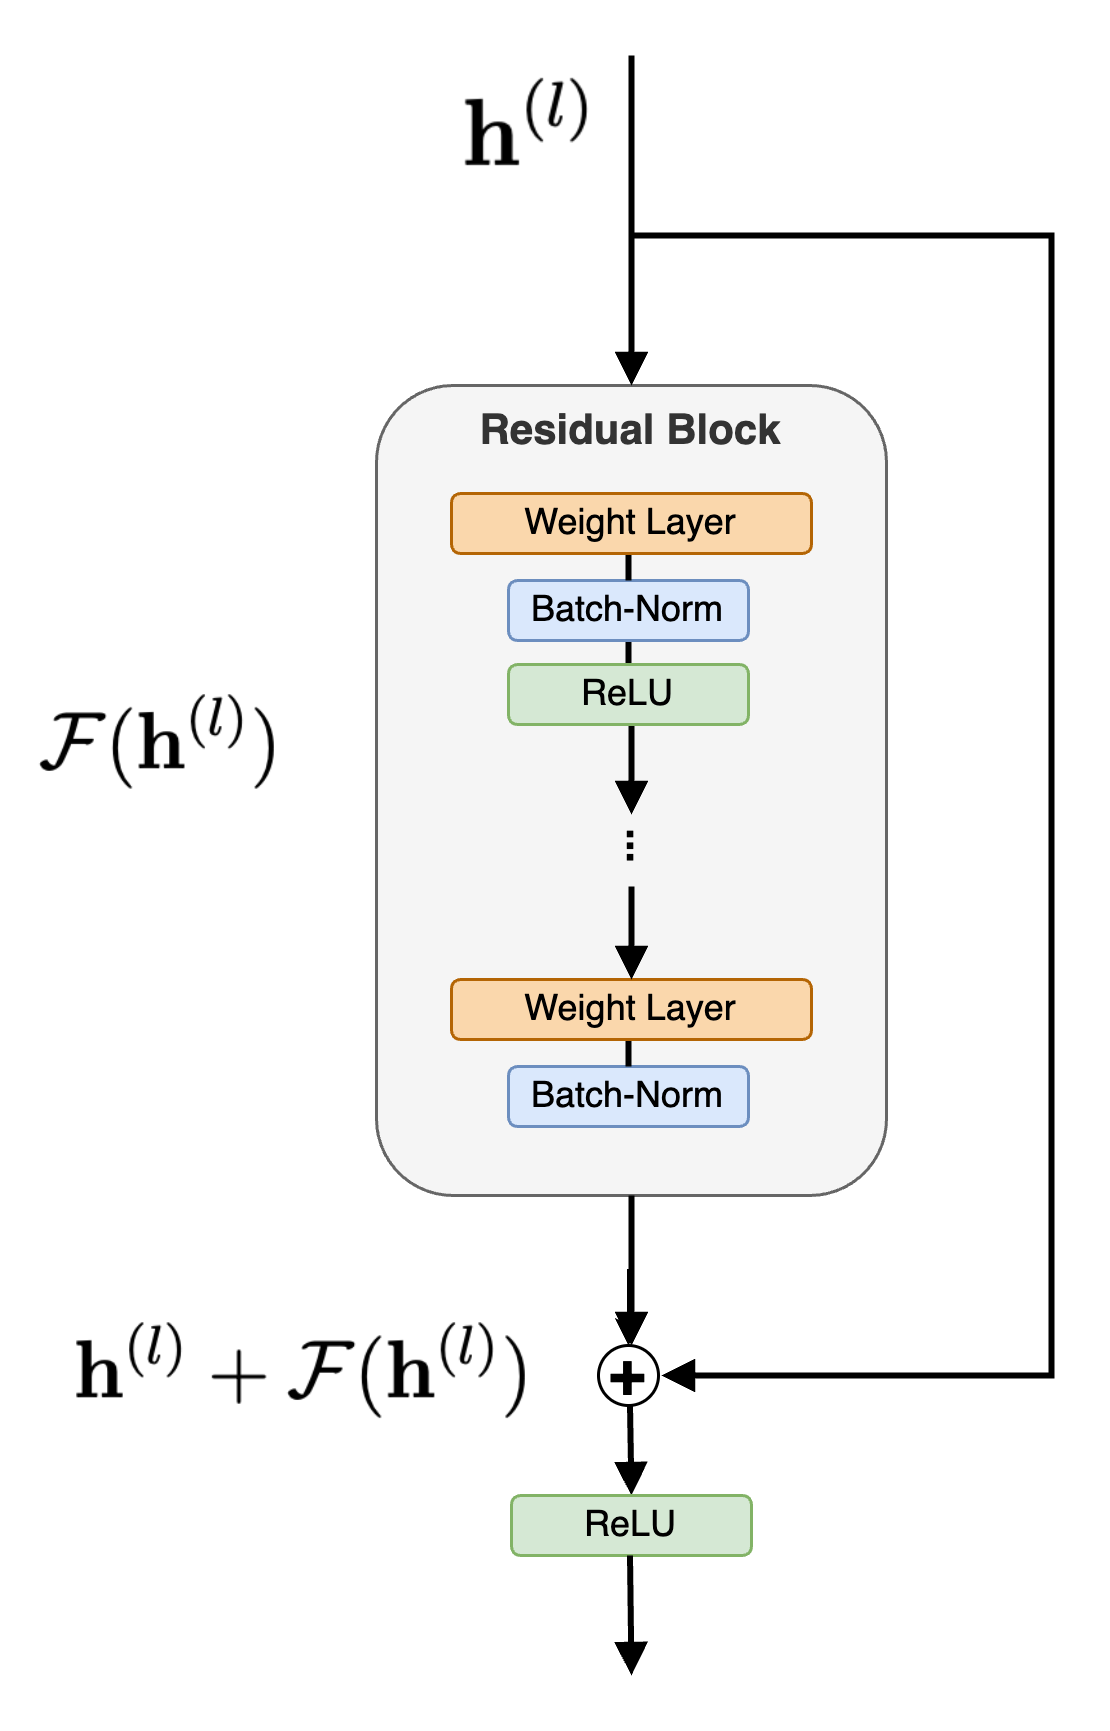
\includegraphics[height = 80mm, width= 55mm]{imgs/resblock.png}
\caption{Residual Block Example (\cite{resnet})}
\label{fig:res_block}
\end{figure}

Many variants of the ResNet have emerged since its initial release in 2015. In 2020, Amazon introduced the ResNeSt model in the paper, \textit{ResNeSt: Split-Attention Networks} \cite{resnest}. This model was built upon the ResNet meta-architecture, and many ResNeSt models contain the same number of layers as the original set of residual networks. However, the network structure was also scaled up to provide even deeper versions, with significantly larger input crop-sizes. For instance, the ResNeSt-269 model has an input crop-size of $416 \times 416$ and has a total of 269 layers. This was particularly attractive for our application to melanoma detection since many of the original images were very large, and we wanted to limit further cropping to minimize additional information loss within our training images.

ResNeSt adopted both the block-style architecture and the identity-skip, or shortcut, connection from the ResNet framework. As before, this mitigated potential vanishing gradient issues. Table 3.2 shows the basic structures of the ResNet-101 and the ResNeSt-101 networks. Since it is not shown in the table, we should note that a $2 \times 2$ average-pooling layer (stride of 2) is also applied to the identity connections in the ResNeSt's transitioning blocks. Average-pooling works very similar to max-pooling in that it simply replaces the value of each pixel by the average of the fixed-size patch surrounding the pixel, instead of the maximum. 

\

\begin{table}[h!]
\centering
\footnotesize 
\renewcommand{\arraystretch}{0.7}
\begin{tabular}{ c | c | c | c } 
\hline
\makecell{\textbf{Layer} \\ \textbf{Name}} & \makecell{\textbf{Output} \\ \textbf{Size}} & \textbf{ResNet-101} & \textbf{ResNeSt-101}\\ 
\hline
\hline
Conv1\_x & $112 \times 112$ & $7 \times 7$, 64, stride 2 & [$3\times 3$]$\times 3$, 64, stride 2\\
\hline
 &  & \multicolumn{2}{c}{$3 \times 3$ max pool, stride 2}\\
\hline
&  & & \\
Conv2\_x & $56 \times 56$ & $\begin{bmatrix} 1 \times 1, 64  \\ 3 \times 3, 64 \\ 1 \times 1, 256 \end{bmatrix} \times 3$ & [\texttt{ResNeSt Block}, 256] $\times 3$\\
&  & & \\
\hline
&  & & \\
Conv3\_x & $28 \times 28$ & $\begin{bmatrix} 1 \times 1, 128  \\ 3 \times 3, 128 \\ 1 \times 1, 512 \end{bmatrix} \times 4$ & [\texttt{ResNeSt Block}, 512] $\times 4$\\
&  & & \\
\hline
&  & & \\
Conv4\_x & $14 \times 14$ & $\begin{bmatrix} 1 \times 1, 256  \\ 3 \times 3, 256 \\ 1 \times 1, 1024 \end{bmatrix} \times 23$ & [\texttt{ResNeSt Block}, 1024] $\times 23$\\
&  & & \\
\hline
&  & & \\
Conv5\_x & $7 \times 7$ & $\begin{bmatrix} 1 \times 1, 512  \\ 3 \times 3, 512 \\ 1 \times 1, 2048 \end{bmatrix} \times 3$ & [\texttt{ResNeSt Block}, 2048] $\times 3$\\
&  & & \\
\hline
Linear & $1 \times 1$ & \multicolumn{2}{c}{average pool, 1000 (fully connected)}\\
\hline  
\end{tabular}
\label{tab:resnet_resnest_archs}
\caption{ResNet-101 and ResNeSt-101 Architecture (\cite{resnet}, \cite{resnest})}
\end{table}


From Table 3.2, we can see the major difference between the ResNet and ResNeSt models lies within the design of the computational blocks. While the ResNet block contains a few convolutional layers, batch normalizations, and ReLU activations, the ResNeSt block is much more involved. Each ResNeSt block has \textit{Split-Attention} sub-blocks that enable channel-wise attention across different subsets of channels. 

We now provide the high-level design of the ResNeSt blocks, as described in the paper, \textit{ResNeSt: Split-Attention Networks} \cite{resnest}. Suppose the input to a given block has shape $(H, W, C)$ where $H$ and $W$ are the spatial dimensions, and $C$ is the number of the channels. At the beginning of each ResNeSt block, the $C$ channels are divided into $K$ groups. Here, $K$ is a tunable hyperparameter referred to as the \textit{cardinality}, and each group is known as a \textit{cardinal group}. Figure 3.7 illustrates this split to cardinal groups.

\begin{figure}[h]
\centering
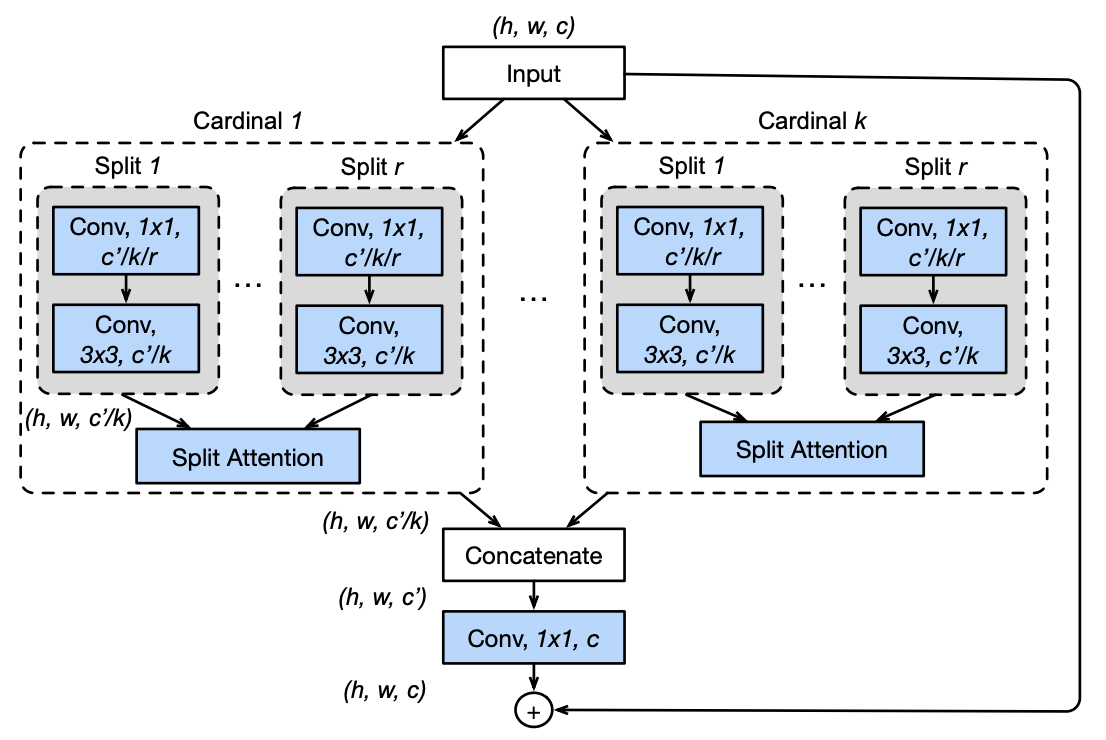
\includegraphics[height = 100mm, width= 130mm]{imgs/resnest_block.png}
\caption{ResNeSt Block (\cite{resnest})}
\label{fig:resnest_block}
\end{figure}

As expected, the block has a shortcut connection on the right-hand side and creates $K$ cardinal groups from the original $C$ input channels. With each cardinal group, the set of $C/K$ channels is further split into $R$ groups. Therefore, the total number of feature groups is $G = KR$. In parallel, two convolutional layers ($1 \times 1$, $3 \times 3$) are then applied to each of the $R$ groups within each cardinal group. The $R$ outputs within each cardinal group are then used together as input for the \textit{Split-Attention block} as shown in Figure 3.8.

\begin{figure}[h]
\centering
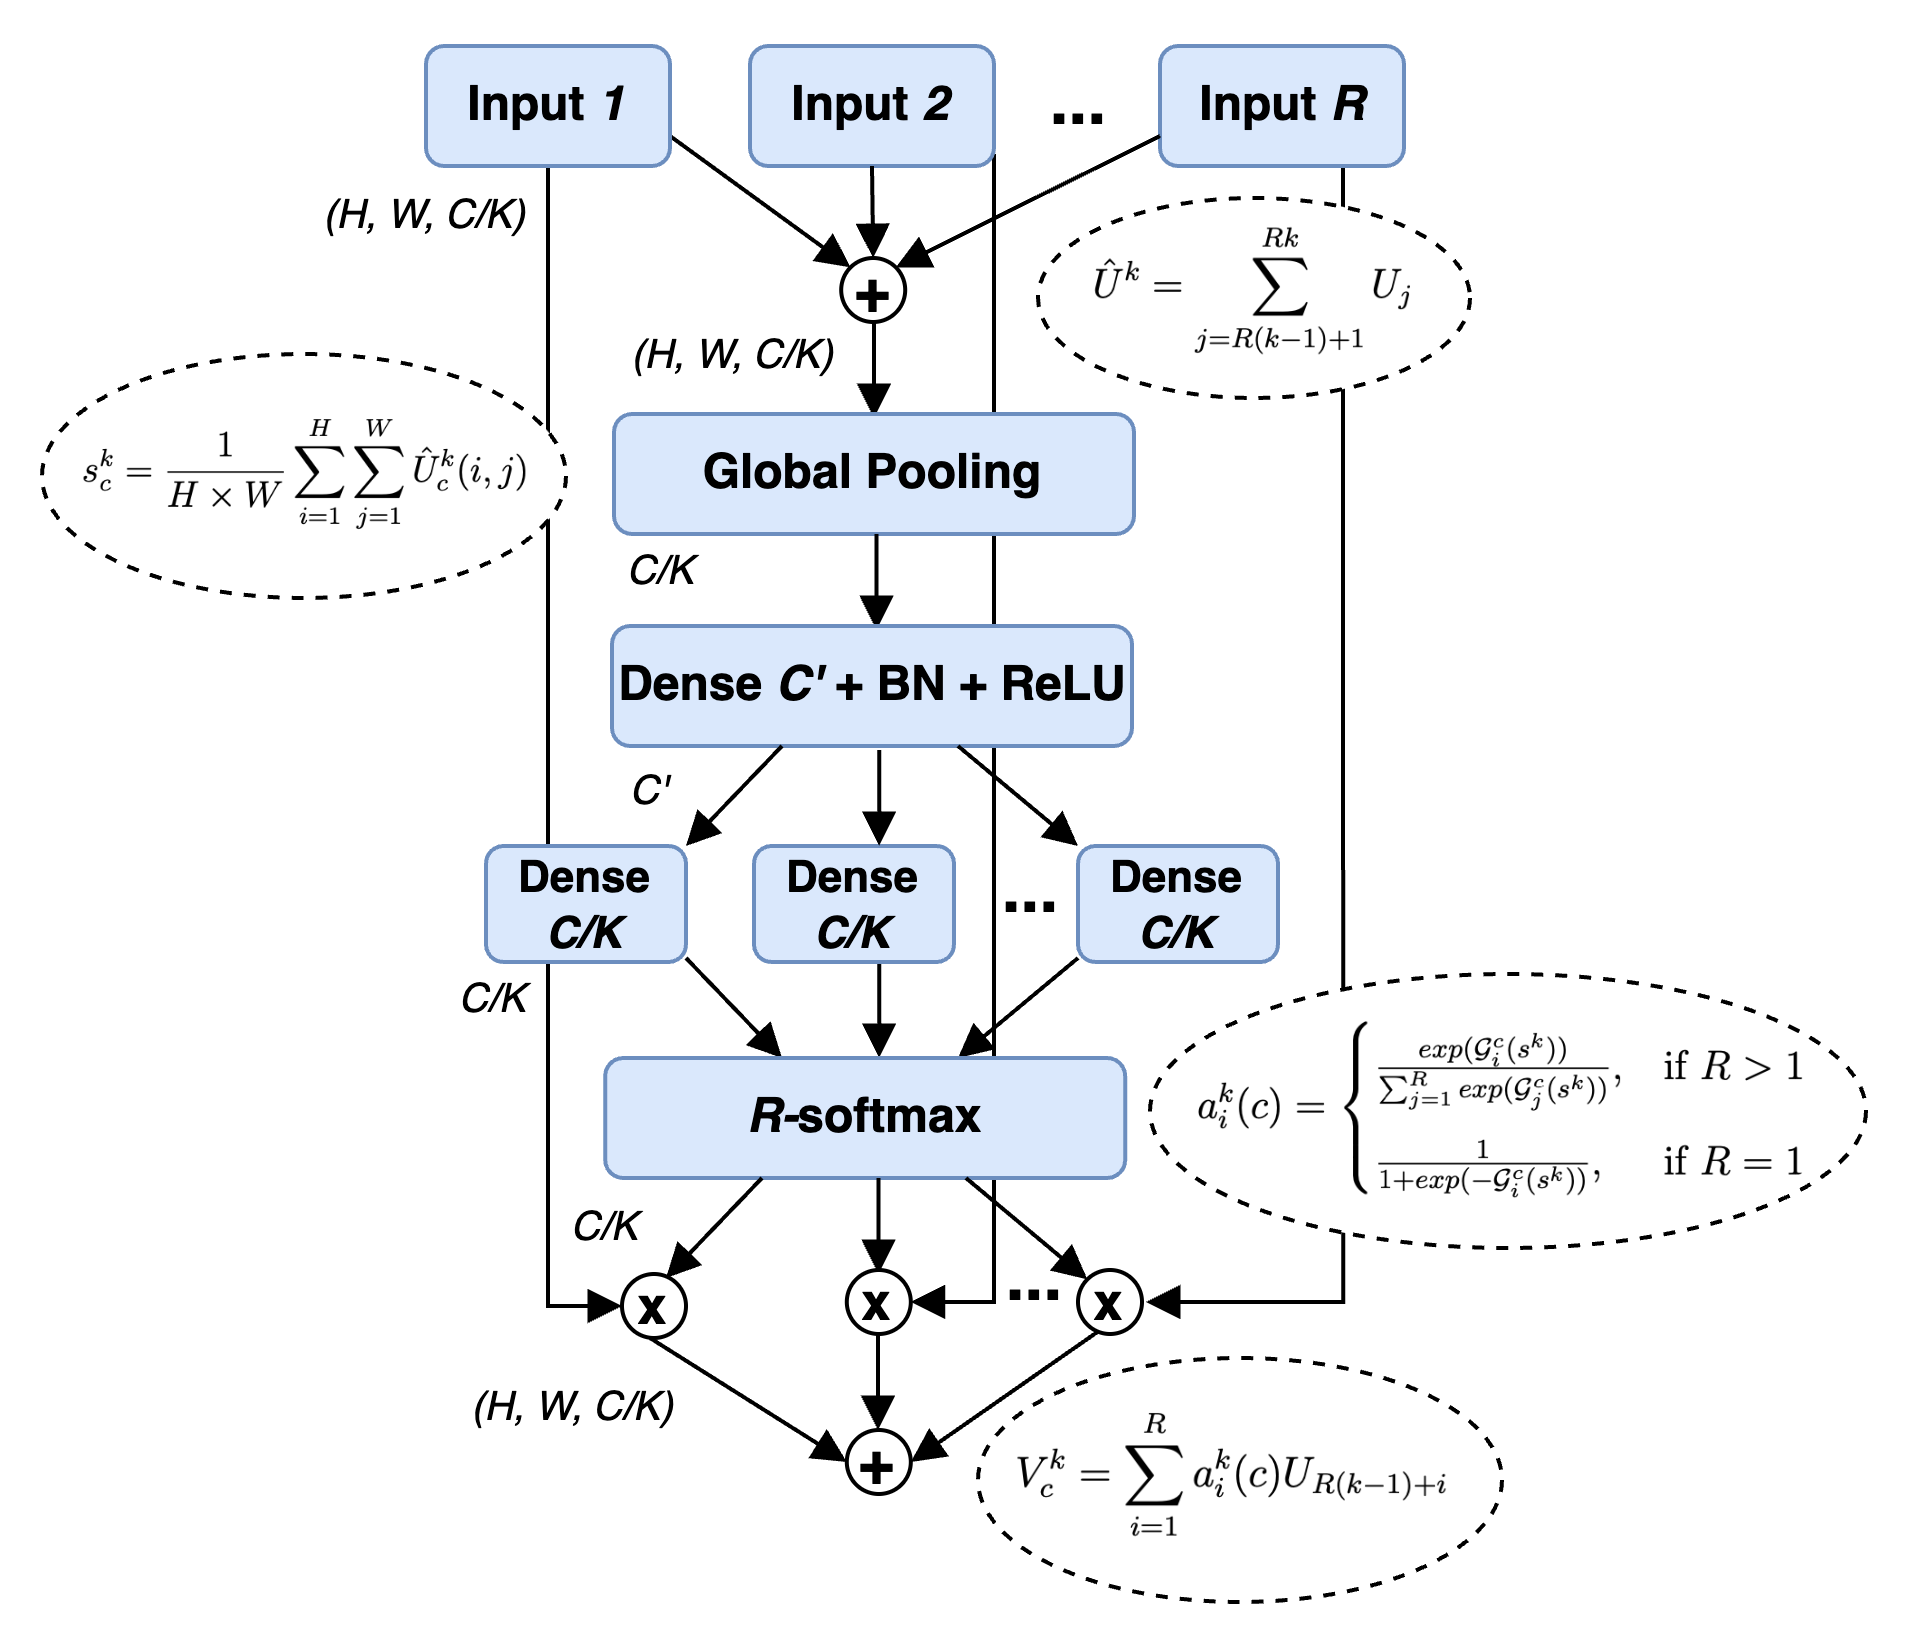
\includegraphics[height = 90mm, width= 100mm]{imgs/split_att.png}
\caption{Split-Attention Block (\cite{resnest})}
\label{fig:split_att_block}
\end{figure}


Let $U_i$ represent the output from the convolutional layers for the $i$th feature group, where $i \in \{1, 2, ..., G \}$. Using these outputs, each split-attention block calculates the combined representation for the $k$th cardinal group: $$\hat{U}^k = \sum_{j = R(k-1)+1}^{Rk} U_j$$ where $\hat{U}^k \in \mathbb{R}^{H \times W \times C/K}$ and $k \in \{1, 2, ..., K\}$. This step is indicated by the fusing together of the $R$ inputs at the very top of the Figure 3.8. Furthermore, each cardinal group's associated channel-wise statistics are then gathered using the global average pooling across the spatial dimensions and may be represented by $s^k \in \mathbb{R}^{C/K}$. The $c$th component of this global pooling vector is calculated as follows: $$s_{c}^{k} = \frac{1}{H \times W} \sum_{i = 1}^{H} \sum_{j = 1}^{W} \hat{U}_{c}^{k}(i, j)$$ The calculation of the global pooling vector, $s^k$, is indicated by the ``Global Pooling'' step shown in Figure 3.8. 

As illustrated, the global pooling vector is ultimately used to compute the weighted fusion of the $k$th cardinal group 
representation, $V^k \in \mathbb{R}^{H \times W \times C/K}$. $V^k$ is computed from channel-wise soft attention such that each channel is a weighted sum over the corresponding $R$ splits. Formally, the $c$th channel is calculated as $$V_{c}^{k} = \sum_{i = 1}^{R} a_{i}^{k}(c) U_{R(k-1) + i}$$ where $a_{i}^{k}(c)$ represents the soft assignment weight such that: \[  a_{i}^{k}(c)= \begin{cases} \frac{exp(\mathcal{G}_{i}^c(s^k))}{\sum_{j=1}^{R} exp(\mathcal{G}_{j}^c(s^k))}, & \text{if } R > 1\\ \frac{1}{1 + exp(-\mathcal{G}_{i}^c(s^k))}, & \text{if } R = 1 \end{cases} \] Here, $\mathcal{G}_{i}^{c}$ denotes a mapping from the global context representation, $s_k$, to an associated weight for the $i$th feature group and $c$th channel. 

Lastly, the cardinal group representations $V^k$, for $k=1, 2, ..., K$, are concatenated along their channel dimensions and a $1 \times 1$ convolutional layer is applied upon return to the ResNeSt block (this is generally performed to restore dimension if reduced at the beginning of the block \cite{resnet}). As illustrated in Figure 3.7, the shortcut connection, $X$, is then added to the concatenated output from the split-attention blocks, $V$. The sum, $V+X$, serves as the final output of the ResNeSt block.

We should note that some of the techniques employed within the split-attention block appear to draw heavily on the multiple-head attention and self-attention mechanisms from the 2017 paper, \textit{Attention Is All You Need} \cite{attention}. Although the transformer model is very different, many of the foundational ideas seem to overlap.

\subsection{Ensemble \#2}

The ResNeSt model has been shown to perform better than the EfficientNet in the accuracy and latency trade-off for image classification problems. Additionally, the ResNeSt model has demonstrated excellent transfer learning results on a variety of well-known public benchmarks. We now discuss the steps we took to leverage this high performing network to pick up on the most important features in our skin lesion images.

As mentioned in the previous section, our second ensemble uses the ResNeSt network to extract the principal features from our image data and uses a standard multi-layer perceptron to find patterns within the patient-level metadata. We used the deepest available network, the \textit{ResNeSt-269}, which has an input crop-size of $416 \times 416$ and has a total of 269 layers. This input size is significantly larger than the maximum crop-size for widely used networks such as those from the ResNet or Inception-Net families. We used this larger network to limit any further cropping of our skin lesion images. Since many of the images were originally very large, further cropping would have lead to unnecessary information loss. In addition, deeper networks generally have a stronger ability to learn features at multiple levels of abstraction, which could lead to a better generalization. As described above, the ResNeSt-269 model stacks several computational blocks containing split-attention operations and shortcut connections, with a variety of intermediate pooling methods (max/average) performed throughout the network. Note that batch normalization was also applied after each block.

After feeding a 3-channel skin lesion image through the ResNeSt-269 model, we will obtain a linear layer with 1000 nodes as output. This output represents the extracted features found from the image. Ideally, the channel-wise attention mechanisms are able to successfully capture the cross-feature interactions that may not be found from the standard convolutional network used in Ensemble \#1. Since the ResNeSt-269 model already contains a deep set of layers, we chose not to attach any additional linear layers to the 1000-node output.

As in Ensemble \#1,  a multi-layer perceptron was also built and trained in parallel to the ResNeSt-269 model. This network also uses the 7 patient-level features as input, then sequentially applies a 256-node linear layer with batch normalization, dropout regularization (with $p=0.2$), and ReLU activation.


\begin{figure}[h]
\centering
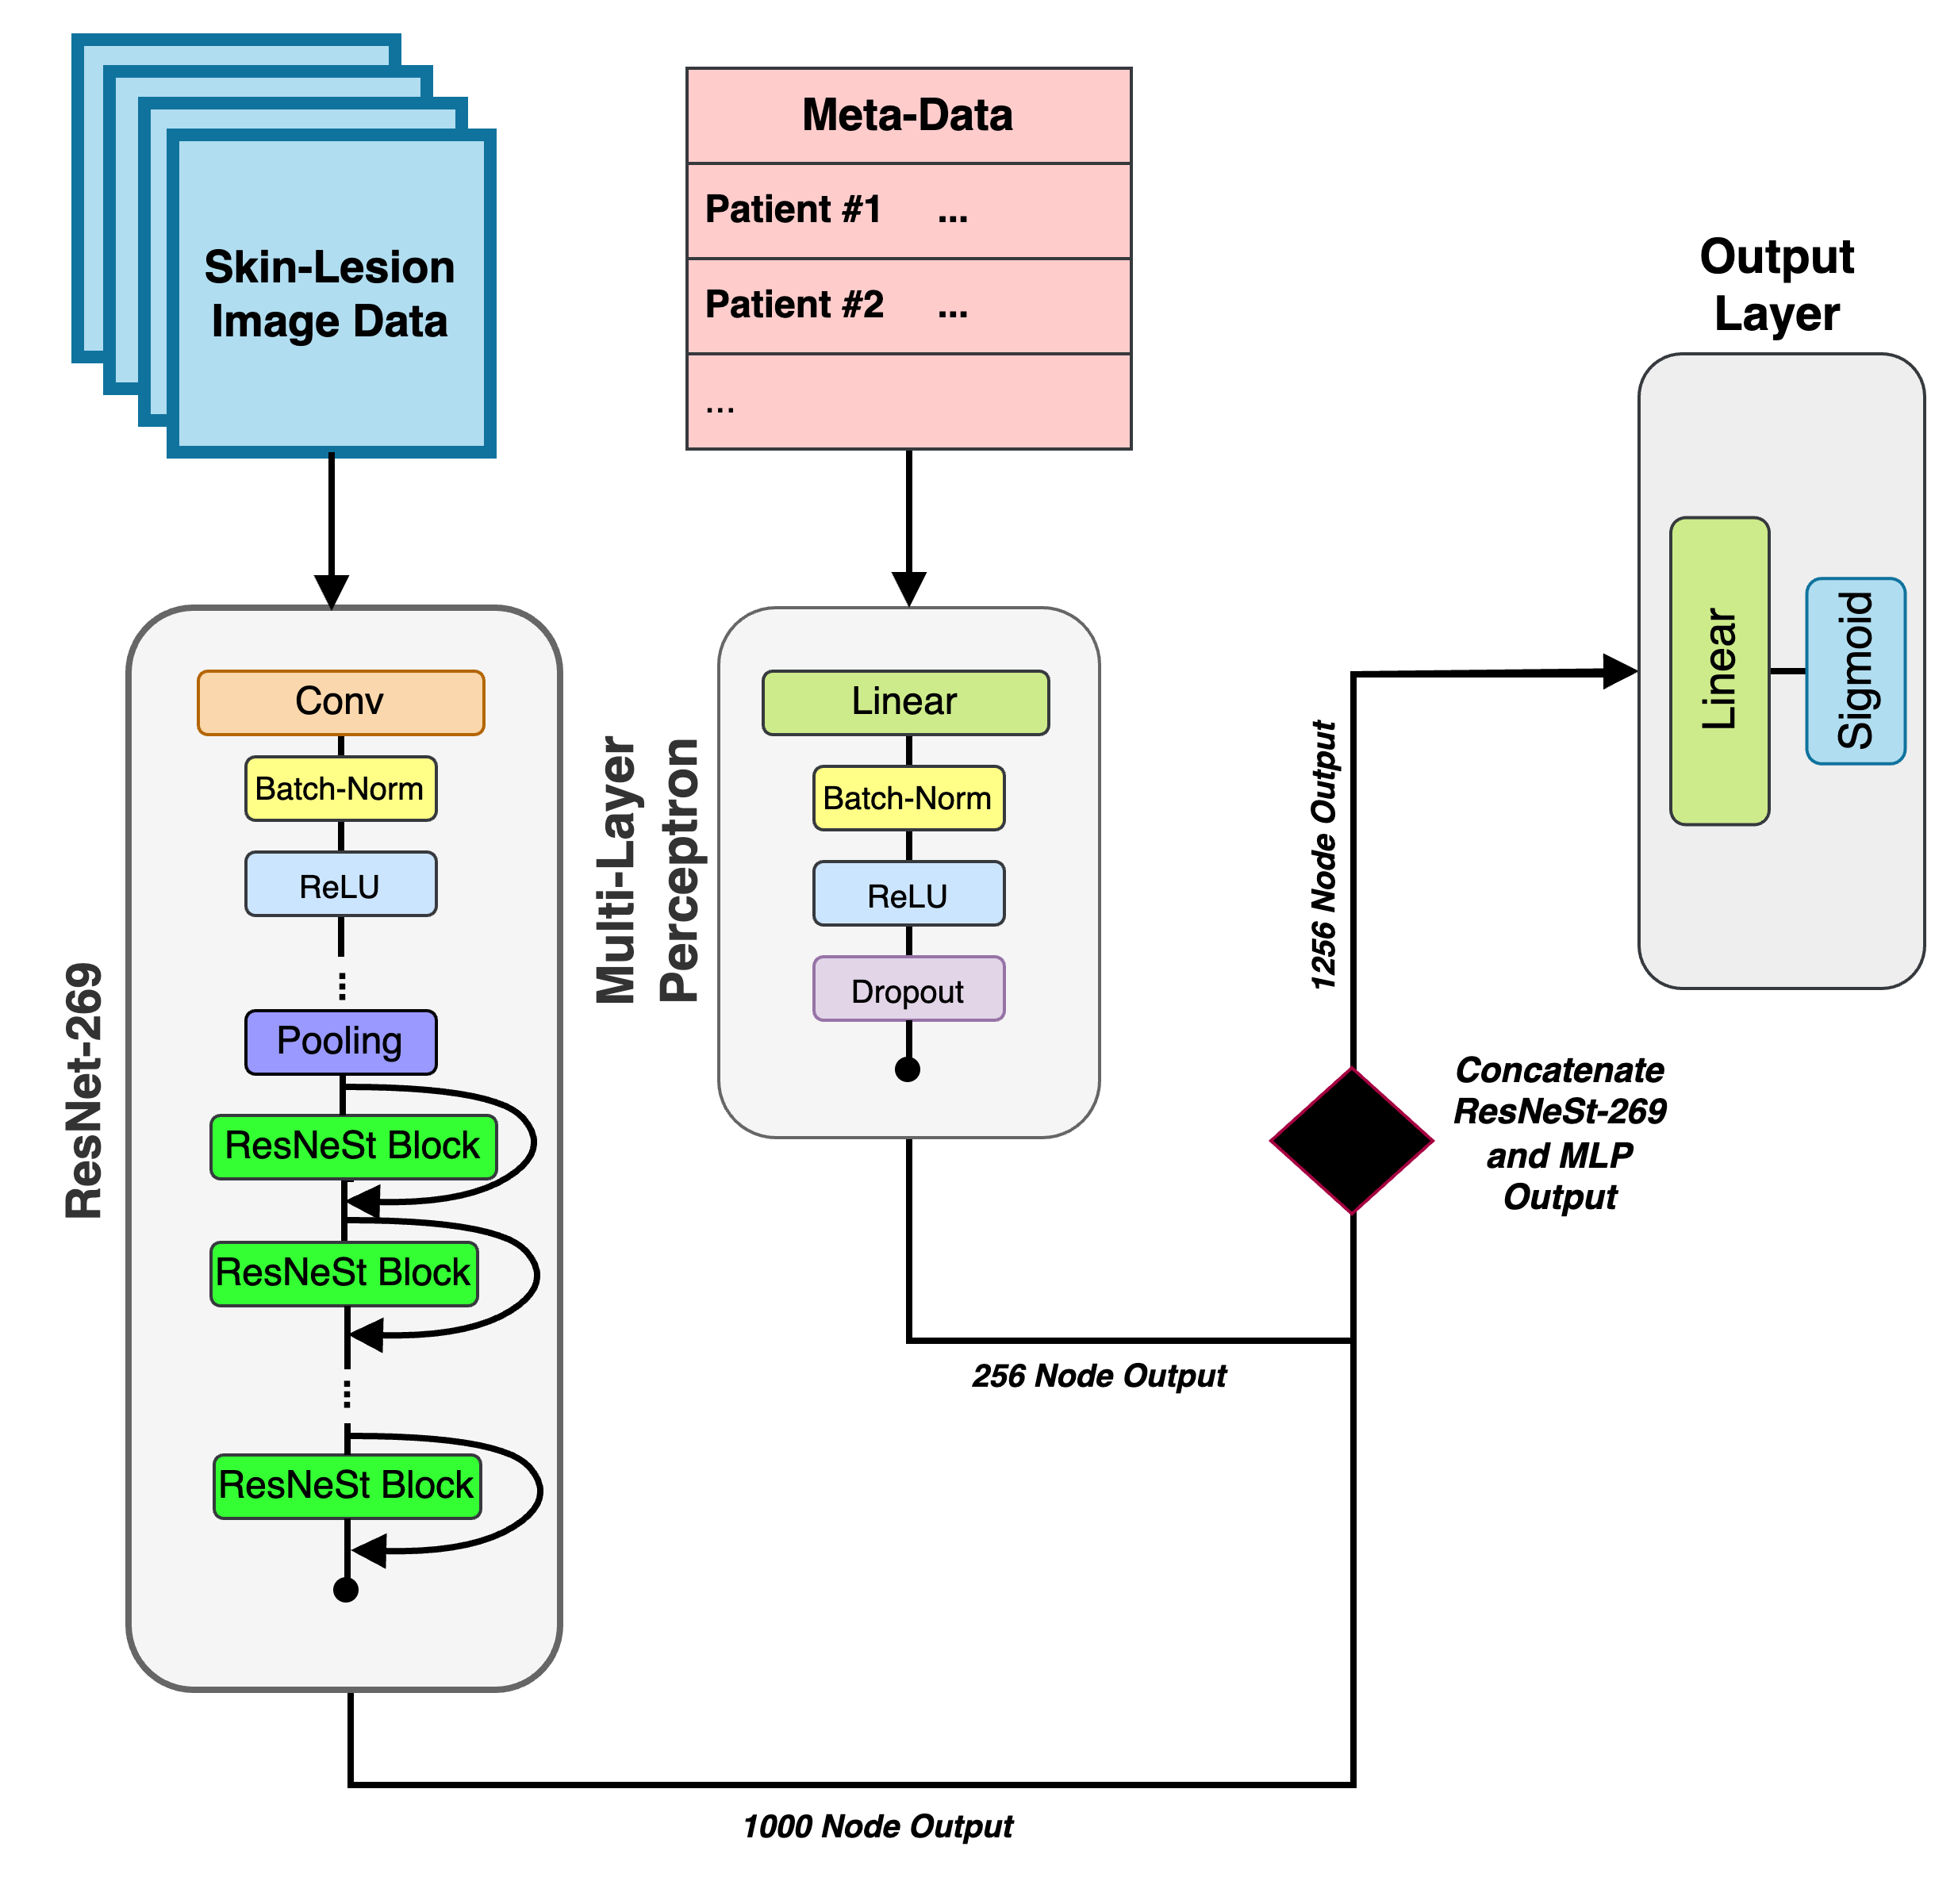
\includegraphics[height = 120mm, width= 140mm]{imgs/ens2_arch.png}
\caption{Multi-Network Ensemble \#2}
\label{fig:ens2_arch}
\end{figure}

Figure 3.9 illustrates how the ResNeSt-269 output was fused together with the multi-layer perceptron output. The concatenated output effectively served as a $1000+256 = 1256$ node linear layer that was then connected to a single output node. As before, we applied the sigmoid function to the output node's final score to provide an estimate for the probability that the skin lesion is malignant.

One of the drawbacks of using such a deep network is that it requires substantial computing resources to train the large number of network parameters. However, pre-trained models that were trained using very powerful computing resources may also be leveraged for our needs. The weights from a network that has \textit{already been trained} for a large-scale, generic, image classification task may be used for our specific application in melanoma detection. This process is known as \textit{transfer learning}. The idea is that if a network has been trained on a large enough, and general enough, dataset, we may take advantage of the learned weights by initializing our network with these pre-trained weights instead of starting with randomly initialized weights. 

In our case, we initialized our ResNeSt-269 model with the pre-trained parameters from the ImageNet dataset \cite{deng2009imagenet}. Instead of holding the pre-trained weights fixed, we decided to \textit{fine-tune} the parameters to our skin lesion images with very small updates to the parameters throughout training. In order to prevent extremely large modifications of the pre-trained weights, we used a smaller learning rate for all parameters associated with the ResNeSt network. However, we used a larger learning rate for the other parameters in Ensemble \#2 since they were still randomly initialized.


\subsection{Evaluation Methods}

To examine and compare the predictive performance of each ensemble, we used our (completely unseen) test data. For each model, we generated predicted probabilities for the test set to obtain visuals such as ROC curves, accuracy plots, sensitivity plots, specificity plots, and false-positive plots. In addition to the visuals, we also computed quantitative measures such as the area under the ROC curves, confusion matrices, and a variety of other performance metrics. 

Although visuals and metrics such as the ROC curve and ROC-AUC consider \textit{all} thresholds, many other measures require a specified probability threshold to generate class predictions. Given that our ensembles attempt to predict the presence of melanoma, the most aggressive form of skin cancer, we aimed to identify a threshold that prioritizes true-positives while not overly accepting too many false-positives. Accepting too many false-positives may compromise the trust in our model's final predictions. In addition, we preferred to optimize our threshold in a way that does not unfairly suffer from the large class imbalance in our data. Therefore, we used the geometric mean of \textit{Sensitivity} (or true-positive rate, $\frac{TP}{TP+FN}$) and \textit{Specificity} (or true-negative rate, $\frac{TN}{TN+FP}$), $$G_{\text{mean}}(t) = \sqrt{\text{Sensitivity} \cdot \text{Specificity}} = \sqrt{\frac{TP \cdot TN }{(TP + FN)(TN + FP)}}$$ to determine an optimal threshold for each model. More specifically, for each model, we found the threshold $t^* \in (0, 1)$ that maximizes the geometric mean, $G_{\text{mean}}(t)$. To retain a completely unseen testing set when evaluating and comparing model performances, we only used the training and validation sets to find $t^*$.

We should note that many ``standard'' performance metrics may not be very useful for our performance assessments. For example, suppose we used test accuracy as a metric for our model's predictive performance. Then, a model that always classifies a skin lesion as benign, regardless of the inputs, would achieve an excellent accuracy of $+98$\% on our imbalanced test set. This measurement would obviously be misleading because such a model would be useless in predicting the presence of melanoma. Therefore, our primary metrics of interest are true-positive rate and true-negative rate as they are not influenced by the large class imbalance within our test data. We used the confusion matrices to compute and output the corresponding sensitivities, specificities, balanced-accuracies, and F2-scores. Balanced-accuracy simply represents the average of the true-positive and true-negative rates, while the F2-score corresponds to the weighted harmonic mean of the precision ($\frac{TP}{TP + FP}$) and sensitivity such that: $$F2_{\text{score}} = \frac{5 \cdot \text{Precision} \cdot \text{Sensitivity}}{4 \cdot \text{Precision} +\text{Sensitivity}}$$ The F2-score represents a single measure for both precision and sensitivity, with slightly more weight on sensitivity than on precision.

\chapter{Results}

\section{Tuning Ensemble \#1}

As we described in Section 3.3.6, Ensemble \#1 uses a standard CNN to process the skin lesion images and a multi-layer perceptron to process the associated patient-level data. Throughout training, we tuned a variety of hyperparameters such as the L2-regularization hyperparameter, $\lambda$, the initial learning rate $\eta \in (10^{-3}, 10^{-1})$, the multiplicative factor of the learning rate decay, $\gamma_{\text{LR}}$, and the total number of training epochs, $M$.

We performed a grid-search to find the optimal set of hyperparameters. In particular, we trained the ensemble with a distinct set of hyperparameters $S^{(k)} = \{\lambda^{(k)}, \eta^{(k)}, \gamma_{\text{LR}}^{(k)}, M^{(k)}\}$ and obtained the ROC-AUC score from the validation data. We trained and validated our ensemble with a total of 10 unique sets of hyperparameters, $S^{(k)}$ for $k=1, 2, ..., 10$, and took the set corresponding to the maximum ROC-AUC, $S^{(\hat k)}$, as the optimal set of hyperparameters. Given our limited computing resources, this repeated process of training and validating was very time-consuming. The process took more than a week to complete, including occasional periods of inactivity. The optimal set of hyperparameters $S^{(\hat k)}$ contained:

\begin{itemize}
    \item L2-regularization hyperparameter: $\hat \lambda = 0.01$
    \item Initial learning rate: $\hat \eta = 0.001$
    \item Learning rate decay factor: $\hat \gamma_{\text{LR}} = 0.5$ (the learning rate is cut in half after each epoch)
    \item Number of epochs: $\hat M=10$
\end{itemize}


\section{Tuning Ensemble \#2}

As we described in Section 3.3.8, Ensemble \#2 uses a ResNeSt-269 model to process the skin lesion images and a multi-layer perceptron to process the associated patient-level data. We tuned a set of hyperparameters similar to Ensemble \#1. However, as mentioned in the previous chapter, we tuned the initial learning rate associated with the ResNeSt model, $\eta_{\text{ResNeSt}}$, separately from the initial learning rate associated with the rest of the ensemble, $\eta_{\text{MLP + Final}}$. This was done because the weights in the ResNeSt model were already pre-trained, so we only wanted to fine-tune them for our application in melanoma detection. Therefore, we tried a variety of initial learning rates between $\eta_{\text{ResNeSt}} \in (10^{-6}, 10^{-5})$ and $\eta_{\text{MLP + Final}} \in (10^{-4}, 10^{-2})$ to find an optimal pair for Ensemble \#2.

Again, we performed a grid-search to find the optimal set of hyperparameters $S^{(\hat k)} = \{\hat \lambda, \hat \eta_{\text{ResNeSt}}, \hat \eta_{\text{MLP + Final}}, \hat \gamma_{\text{LR}}, M^{(k)}\}$ using the ROC-AUC scores from the validation data. We trained and validated this ensemble with a total of 15 unique sets of hyperparameters, $S^{(k)} = \{\lambda^{(k)}, \eta_{\text{ResNeSt}}^{(k)}, \eta_{\text{MLP+Final}}^{(k)}, \gamma_{\text{LR}}^{(k)}, M^{(k)}\}$, for $k=1, 2, ..., 15$. Since the ResNeSt-269 model contained over 100 million parameters alone, training Ensemble \#2 required significantly more time than Ensemble \#1. In total, the entire process of training required about 2 weeks, including occasional periods of inactivity. In this case, the optimal set of hyperparameters $S^{(\hat k)}$ contained:

\begin{itemize}
    \item L2-regularization hyperparameter: $\hat \lambda = 0$ (No L2-regularization applied)
    \item Initial learning rate for ResNeSt-269 parameters: $\hat \eta_{\text{ResNeSt}} = 3 \times 10^{-5}$
    \item Initial learning rate for all other parameters: $\hat \eta_{\text{MLP+Final}} = 1 \times 10^{-3}$
    \item Learning rate decay factor: $\hat \gamma_{\text{LR}} = 0.1$
    \item Number of epochs: $\hat M=10$
\end{itemize}

We should note that the optimal hyperparameters listed for Ensemble \#1 and Ensemble \#2 were ultimately used to re-train the models with the combined training and validation data prior to obtaining any test results.


\section{Evaluation and Comparison}

In this final results section, we use the dedicated test data to assess and compare the overall predictive performance of both
multi-network ensembles. We started by examining the metrics of interest, true-positive rate and true-negative rate, computed at all possible thresholds. Figure 4.1 displays the sensitivity and specificity scores across the range of thresholds, $t \in (0, 1)$.

\begin{figure}[hbt!]
\hspace*{\fill}
\centering
\subcaptionbox{}{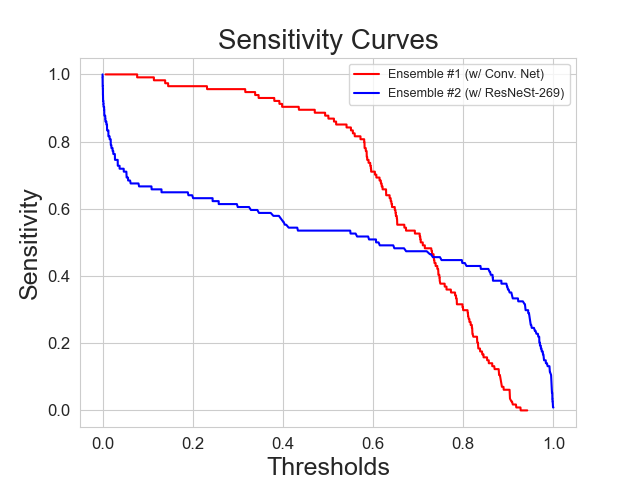
\includegraphics[height = 70mm, width=80mm]{imgs/results_sens.png}}\hspace{0em}
\subcaptionbox{}{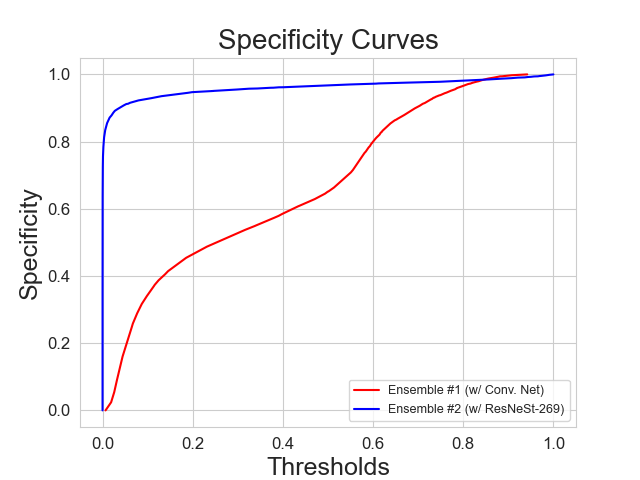
\includegraphics[height = 70mm, width=80mm]{imgs/results_spec.png}}
\hspace*{\fill}
\label{fig:sens_spec}
\vspace{0cm}
\caption{True-Positive Rates and True-Negative Rates for Ensembles \#1 \& \#2}
\end{figure}


As mentioned in Section 3.3.9, since our ensembles are ultimately predicting the presence of a life-threatening condition, a false-negative is far more dangerous than a false-positive. Ideally, we want our ensembles to have the greatest possible true-positive rate without compromising the overall ``trust'' in its classifications. Therefore, our goal was to maximize the sensitivity without dropping the specificity too much. Figure 4.1 indicates that there may exist a distinct range of thresholds for each model that could accomplish this goal. From Figure 4.1(a) and Figure 4.1(b), we can see that the optimal threshold lies within $t \in (0.45, 0.75)$ for Ensemble \#1 since there appears to be the best balance of sensitivity and specificity in this range. For Ensemble \#2, Figure 4.1(a) indicates a sharp and sudden drop in sensitivity within a lower range of thresholds. However, Figure 4.1(b) shows an equally sharp and sudden \textit{increase} in specificity within the same range of lower thresholds. Therefore, we can see that the optimal threshold lies within $t \in (0, 0.05)$ for Ensemble \#2.

The geometric mean of the sensitivity and the specificity was then used to find the optimal threshold, $t^*$, for each model. We evaluated $G_{\text{mean}}(t)$ at a variety of different thresholds $t \in (0, 1)$, and stored the threshold that maximized $G_{\text{mean}}(t)$. Using the optimal thresholds for each model, we created the following performance metrics and confusion matrices from our test set.

\

\begin{table}[h!]
\centering
\footnotesize 
\begin{tabular}{| c | c | c | c | c | c | c |} 
\hline
\textbf{Model} & $\mathbf{t^*}$ & $\mathbf{G_{\text{mean}}}$ & \textbf{Sensitivity} & \textbf{Specificity} & \makecell{\textbf{Balanced} \\ \textbf{Accuracy}} & $\mathbf{F2_{\text{score}}}$ \\ 
\hline
\hline
\makecell{Ensemble \#1 \\ (w/ Conv. Net)} & 0.580 & 0.781 & 0.798 & 0.765 & 0.782 & 0.105\\
\hline
\makecell{Ensemble \#2 \\ (w/ ResNeSt-269)} & 0.003 & 0.853 & 0.895 & 0.813 & 0.853 & 0.287\\
\hline  
\end{tabular}
\label{tab:mods_metrics}
\caption{Performance Metrics Using the $G_{\text{mean}}(t)$ Maximizer, $t^*$}
\end{table}

\begin{table}[hbt!]
\footnotesize 
\hspace{-1.3em}
\begin{subtable}{.5\linewidth}\centering
{\begin{tabular}{cc|c|c|c|}
&\multicolumn{1}{c}{}&\multicolumn{3}{c}{\textbf{Predicted}}\\
&\multicolumn{1}{c}{}&\multicolumn{1}{c}{\textbf{Benign}}
&\multicolumn{1}{c}{\textbf{Malignant}}
&\multicolumn{1}{c}{\textbf{Total}}\\
\cline{3-5}
\multicolumn{1}{c}{\multirow{3}{*}{\rotatebox{90}{\textbf{Actual}}}}
&\textbf{Benign} &4981 & 1531 &  6512\\
\cline{3-5}
&\textbf{Malignant} &23 & 91 & 114\\
\cline{3-5}
&\textbf{Total} &5004 & 1622 &\\
\cline{3-5}
\end{tabular}}
\caption{Ensemble \#1 (w/ Conv. Net)}
\end{subtable}\hspace{1em}
\begin{subtable}{.5\linewidth}\centering
{\begin{tabular}{cc|c|c|c|}
&\multicolumn{1}{c}{}&\multicolumn{3}{c}{\textbf{Predicted}}\\
&\multicolumn{1}{c}{}&\multicolumn{1}{c}{\textbf{Benign}}
&\multicolumn{1}{c}{\textbf{Malignant}}
&\multicolumn{1}{c}{\textbf{Total}}\\
\cline{3-5}
\multicolumn{1}{c}{\multirow{3}{*}{\rotatebox{90}{\textbf{Actual}}}}
&\textbf{Benign} & 5293 &  1219 &  6512\\
\cline{3-5}
&\textbf{Malignant} & 12 & 102 & 114\\
\cline{3-5}
&\textbf{Total} &5305 & 1321 &\\
\cline{3-5}
\end{tabular}}
\caption{Ensemble \#2 (w/ ResNeSt-269)}
\end{subtable}
\label{tab:conf_mats}
\caption{Confusion Matrices For Both Multi-Network Ensembles}
\end{table}
    
From the performance metrics and confusion matrices, we can see that both models demonstrate an excellent classification performance. However, the improvement from the ResNeSt-269 model in Ensemble \#2 is very apparent. Using the deep split-attention network to process the skin lesion images rather than a generic convolutional neural network has shown to drastically improve every metric listed in Table 4.1. Most notably, we can see that the balanced accuracy increases by over 7\% when using Ensemble \#2! This indicates that Ensemble \#2 was able to successfully leverage the ResNeSt-269 architecture to extract the most important features from the skin lesion images.

For a more general assessment and comparison across all possible thresholds, we also used the testing data to compute the ROC curves for each model (shown below) and their associated ROC-AUCs.

\begin{figure}[hbt!]
\makebox[\linewidth][c]{
\footnotesize 
\centering
\hspace{2em}
\vspace{0cm}
\subcaptionbox{}{\hspace{1em}\vspace{1.1cm}\begin{tabular}{| c | c |} 
\hline
& \\
\textbf{Model} & \makecell{\textbf{ROC} \textbf{AUC}} \\ 
& \\
\hline
& \\
\makecell{Ensemble \#1 \\ (w/ Conv. Net)} & 0.852\\
& \\
\hline
& \\
\makecell{Ensemble \#2 \\ (w/ ResNeSt-269)} & 0.929\\
& \\
\hline
\end{tabular}}\hspace{1em}
\subcaptionbox{}{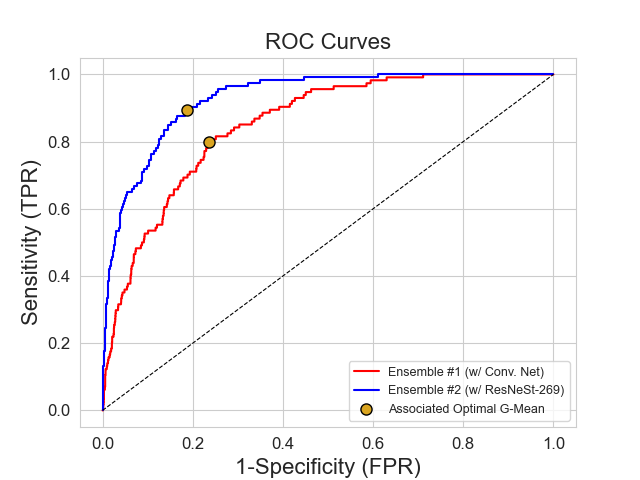
\includegraphics[height = 95mm, width=115mm]{imgs/results_roc.png}} 
\hspace*{\fill}
}
\label{fig:roc}
\caption{ROC-AUC and ROC Curves for Ensemble's \#1 \& \#2}
\end{figure}


Although it is difficult to evaluate the models visually from Figure 4.2(b), from the plot and the associated table of ROC-AUC scores, we can see that both ensembles demonstrated outstanding predictive performance across the entire range of thresholds. They each exhibit an ability to successfully classify whether or not the skin lesion is benign or malignant, and they appear to produce predictive results significantly better than a model that purely guesses (which is displayed by the black dashed line).

The associated ROC-AUCs from Figure 4.2(a) also tell us that the ensemble using the ResNeSt-269 model for feature extraction was able to detect the presence of melanoma better than the ensemble using the generic CNN, across the entire range of thresholds. That is, at each threshold $t \in (0, 1)$, the aggregate score of sensitivity and specificity was the same or better for Ensemble \#2 than it was for Ensemble \#1. Using the split-attention network increased the total area under the ROC curve by approximately 9\%. This provides further evidence suggesting that the second ensemble model was able to successfully leverage the channel-wise attention design within the ResNeSt network to extract the most important features and most relevant cross-feature interactions from the skin lesion images.

\chapter{Conclusion and Future Work}

We began this paper with a brief introduction to the ISIC 2020 dataset. We then performed a thorough exploratory data analysis for both skin lesion images and patient-level metadata. The design and implementation of the two multi-network ensembles used to detect the presence of melanoma were then discussed in detail. Ensemble \#1 used a generic convolutional neural network for the skin lesion images and a multi-layer perceptron model for the patient-level metadata. Ensemble \#2 used a split-attention network architecture from the 269-layer ResNeSt model to extract the most important features from the image data, and also used the multi-layer perceptron model for the metadata. PyTorch was used for the implementation of each model \cite{NEURIPS2019_9015}

The test results demonstrated powerful predictive performance from both models. In fact, both ensembles achieved an outstanding ROC-AUC score over 0.85 and a balanced accuracy over 75\% (using their optimal thresholds). However, the test results also indicated an improvement in the predictive power of Ensemble \#2 when compared to Ensemble \#1. The ResNeSt's architecture was shown to significantly increase the sensitivity, specificity, and the area under the ROC curve. Therefore, Ensemble \#2 was able to successfully leverage the channel-wise attention from the ResNeSt blocks, as well as the deep design of the ResNeSt-269 architecture, to extract the most important features and the most relevant cross-feature interactions from the skin lesion images. The evidence suggests that the extracted features were highly significant for predicting the presence of melanoma.

In conclusion, using the split-attention network within our ensemble model has demonstrated excellent predictive performance in detecting melanoma. The classification ability is comparable to many of the most powerful models used in melanoma detection today \cite{EffNet_MelDet}. 

Future work could involve alternative models or pre-processing techniques for the patient-level metadata. For instance, some form of feature selection or a tree-based model for the metadata may lead to a better performance from our ensemble. Additionally, future work could also directly compare the performances between ensembles using other well known pre-trained networks, such as the \textit{EfficientNet}, for the image data. Using the same training and testing split would ensure a fair comparison of the models.

\bibliography{bib/resnest_melanoma_detection.bib}    % bibliography references
\bibliographystyle{uclathes}


\end{document}